\documentclass[10pt]{mypackage}

% sans serif font:
%\usepackage{cmbright}
%\usepackage{sfmath}
%\usepackage{bbold} %better blackboard bold

%serif font + different blackboard bold for serif font
\usepackage{newpxtext,eulerpx}
\renewcommand*{\mathbb}[1]{\varmathbb{#1}}
\renewcommand*{\hbar}{\hslash}

\pagestyle{fancy} %better headers
\fancyhf{}
\rhead{Avinash Iyer}
\lhead{Ordinary Differential Equations: Homework 11}

\setcounter{secnumdepth}{0}

\begin{document}
\RaggedRight
\section{Part 1}%
\subsection{3.5, Problem 18}%
\begin{enumerate}[(a)]
  \item 
    \begin{align*}
      \det \begin{pmatrix}2-\lambda & 4 \\ 3 & 6-\lambda\end{pmatrix} &= \left(\lambda - 2\right)\left(\lambda - 6\right) - 12\\
      \lambda\left(\lambda - 8\right) &= 0,
    \end{align*}
    meaning $\lambda = 0,8$.
  \item The eigenvector for $\lambda = 0$ is
    \begin{align*}
      2x &= -4y\\
      x &= -2y\\
      \vec{v}_1 &= \begin{pmatrix}-2 \\ 1\end{pmatrix},
    \end{align*}
    and the eigenvector for $\lambda = 8$ is
    \begin{align*}
      2x + 4y &= 8x\\
      4y &= 6x\\
      y &= \frac{2}{3}x\\
      \vec{v}_2 &= \begin{pmatrix}3\\2\end{pmatrix}.
    \end{align*}
  \item 
    \begin{center}
      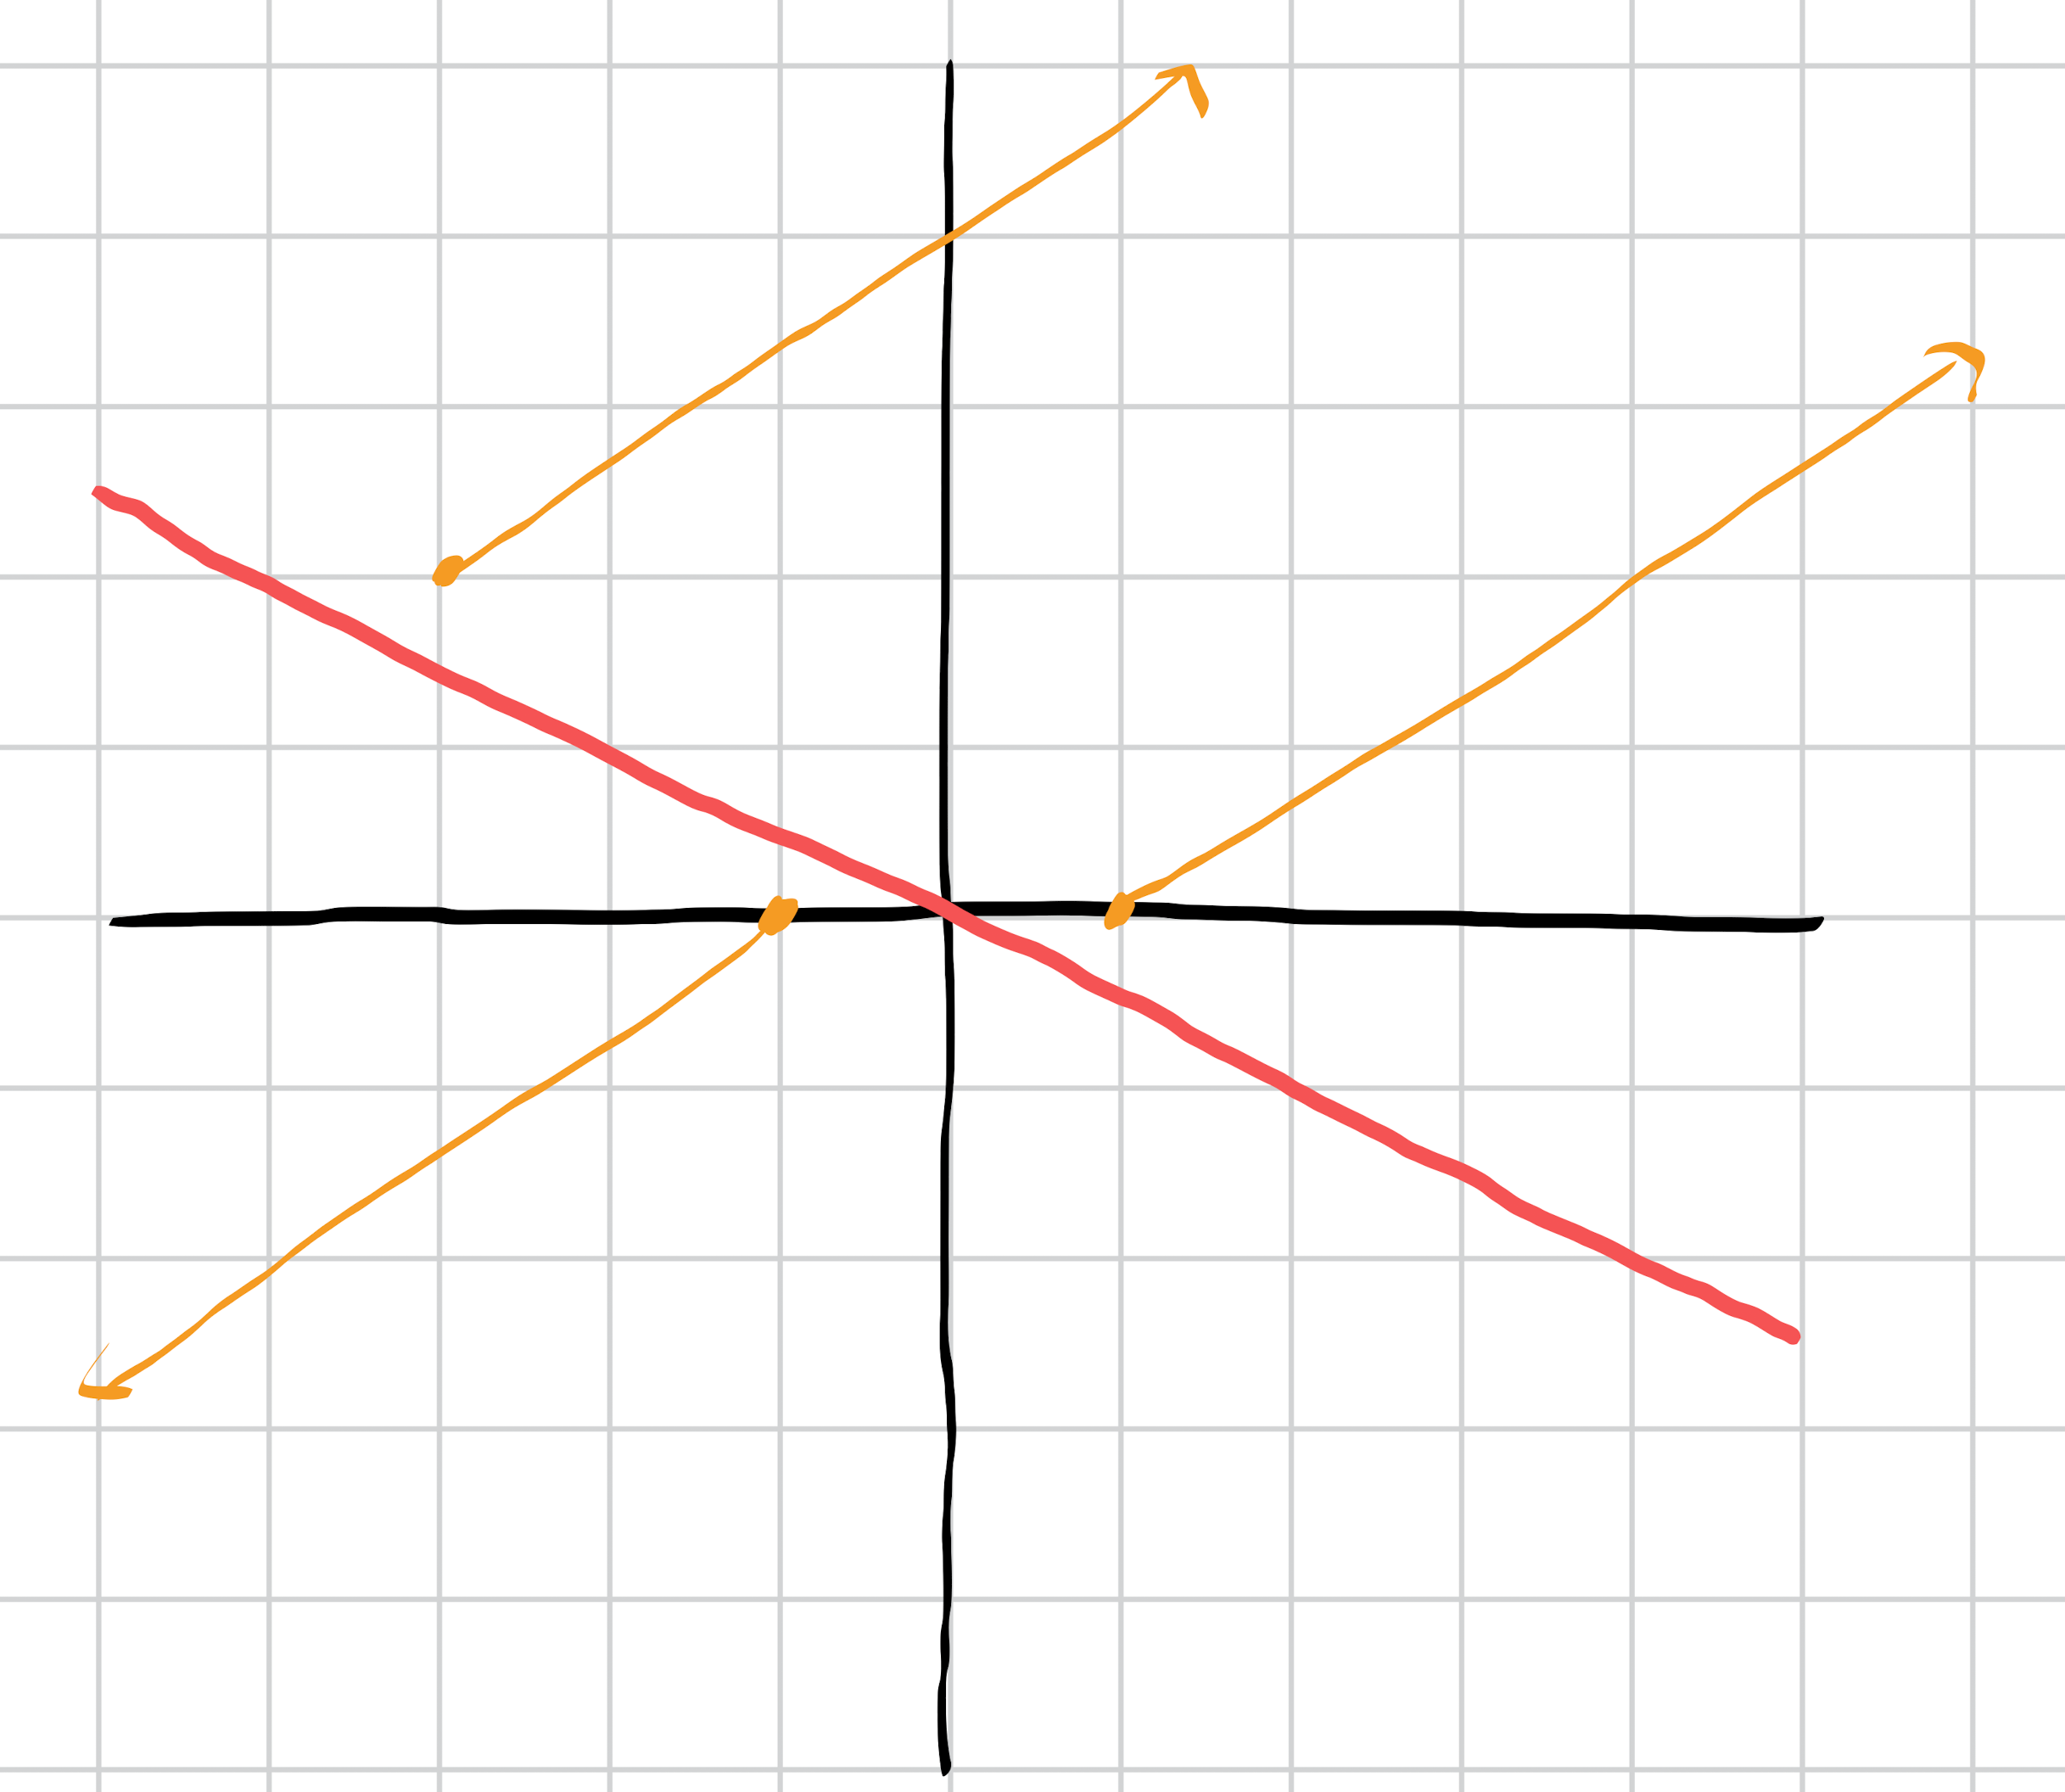
\includegraphics[width=7cm]{images/3_5_18c.png}
    \end{center}
  \item 
    \begin{center}
      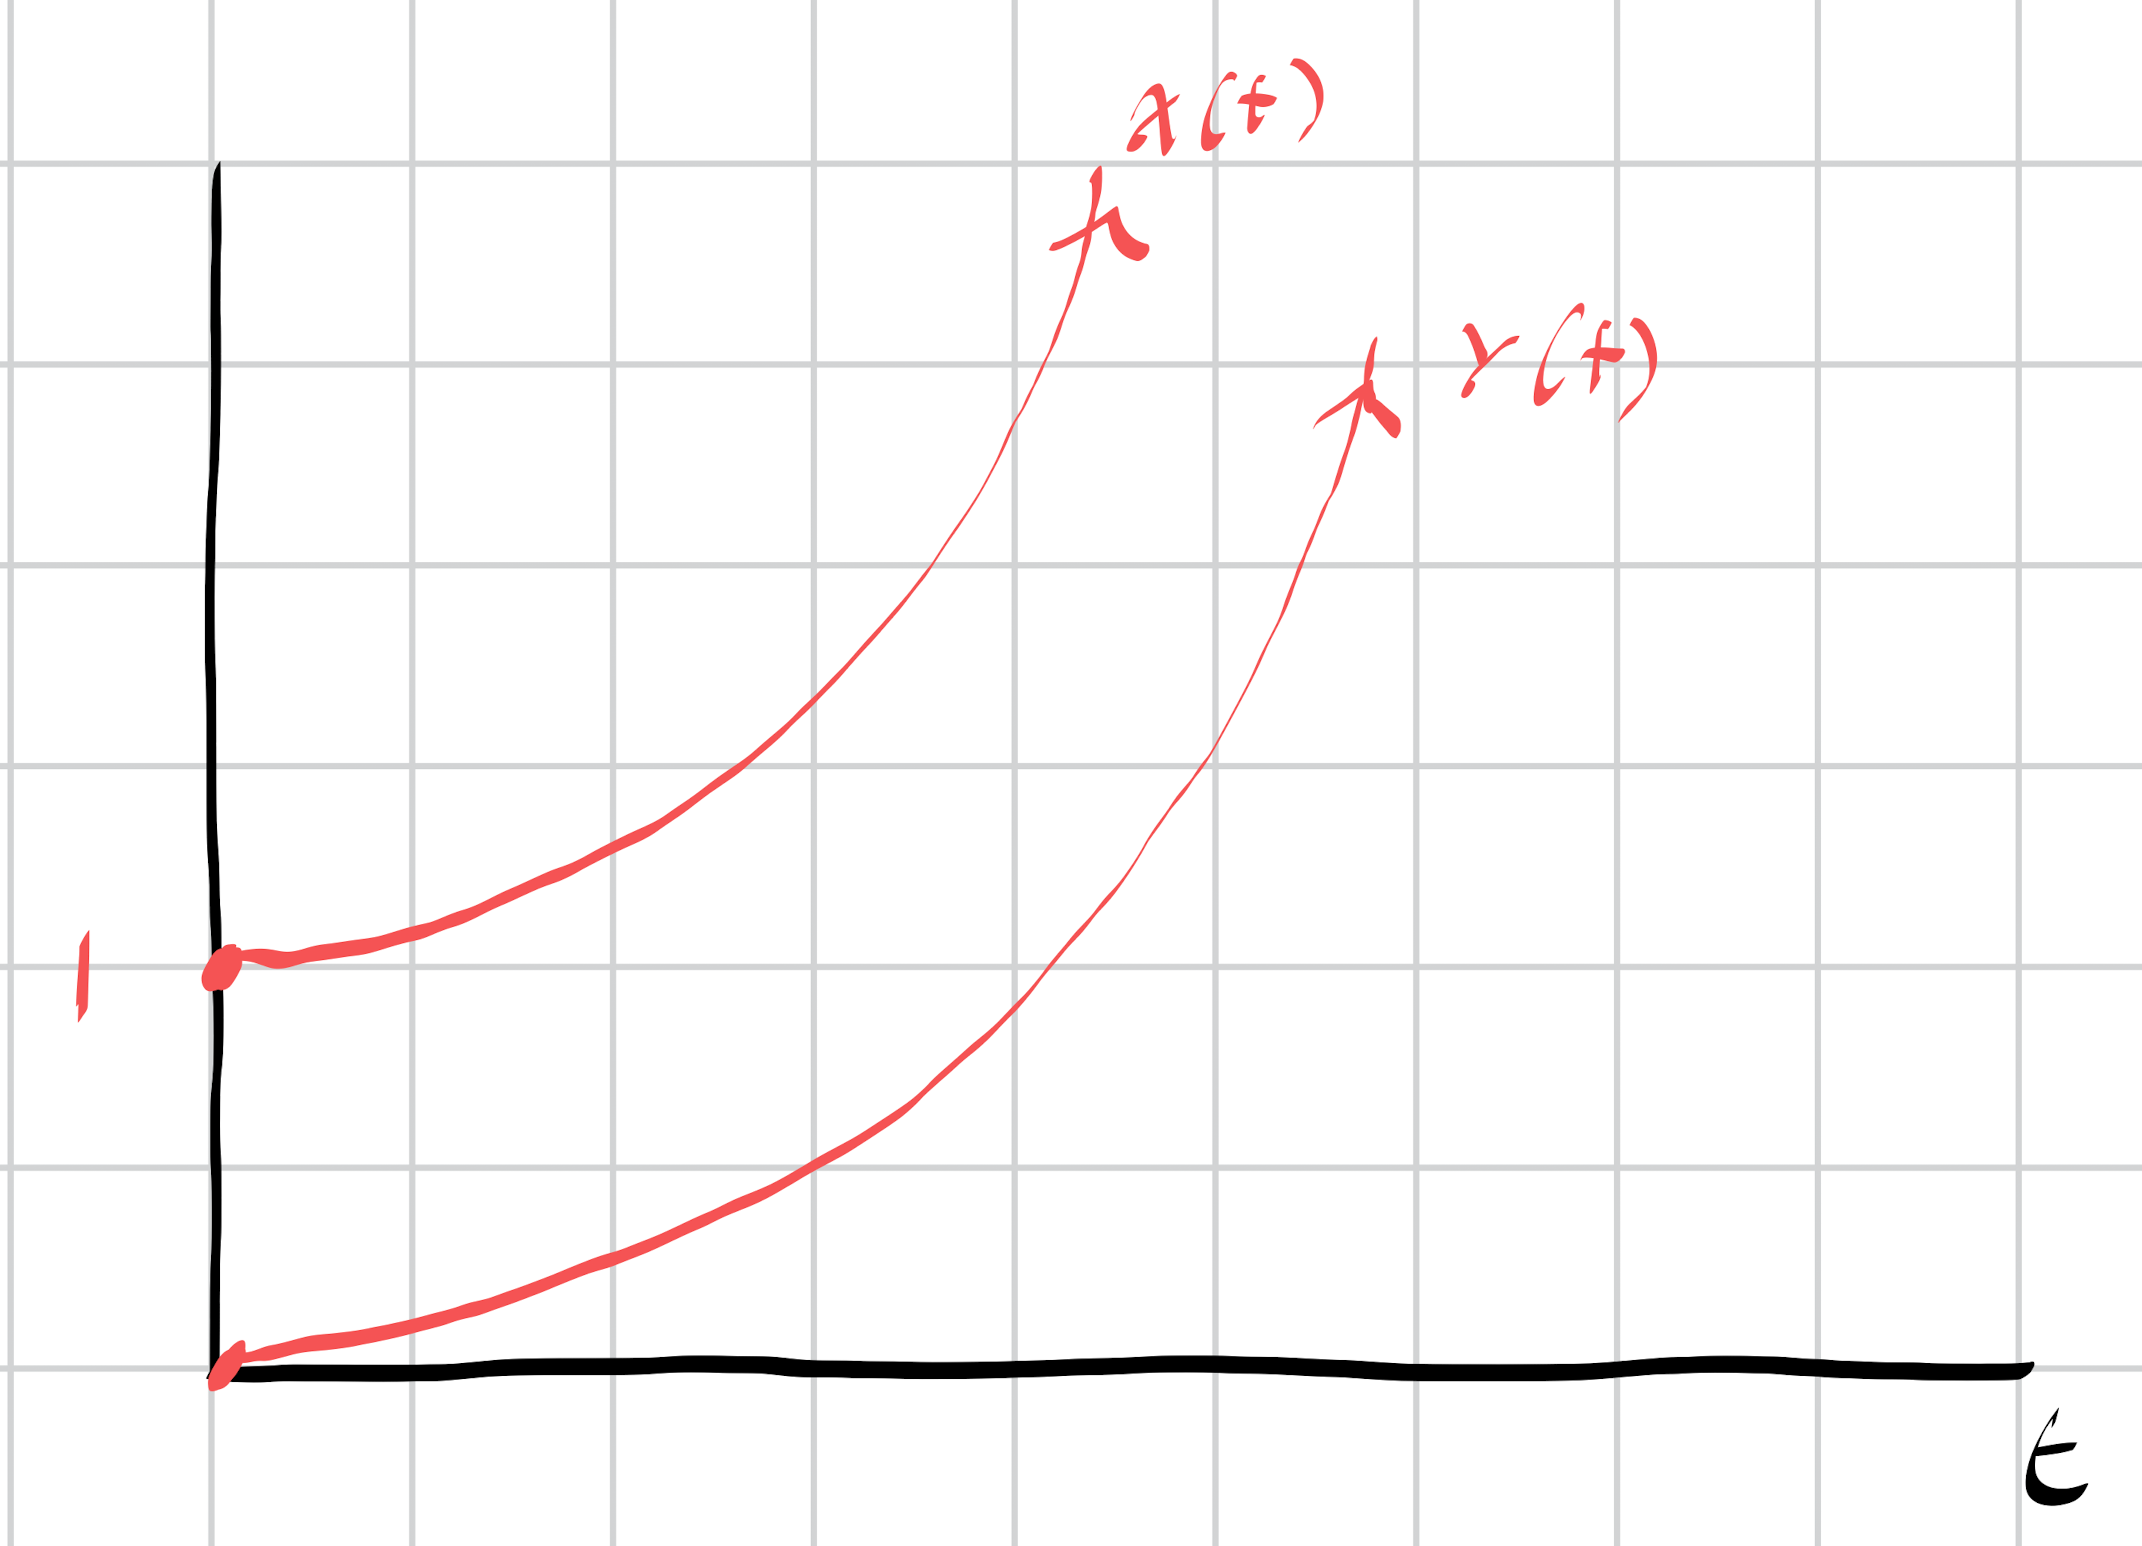
\includegraphics[width=7cm]{images/3_5_18d.png}
    \end{center}
  \item 
    \begin{align*}
      \vec{Y}(t) &= k_1 \begin{pmatrix}-2\\1\end{pmatrix} + k_2e^{8t} \begin{pmatrix}3\\2\end{pmatrix}.
    \end{align*}
  \item Solving for the initial condition, we have
    \begin{align*}
      1 &= -2k_1 + 3k_2\\
      0 &= k_1 + 2k_2,
    \end{align*}
    so $k_1 = -2k_2$, and
    \begin{align*}
      1 &= 7k_2\\
      k_2 &= \frac{1}{7}\\
      k_1 &= -\frac{2}{7}.
    \end{align*}
    Thus, we get
    \begin{align*}
      \vec{Y}_1(t) &= \frac{1}{7} \begin{pmatrix}-2\\1\end{pmatrix} -\frac{2}{7}e^{8t} \begin{pmatrix}3\\2\end{pmatrix}.
    \end{align*}
\end{enumerate}
\subsection{3.5, Problem 21 (a)}%
There are two repeated eigenvalues at $0$. All solutions are of the form
\begin{align*}
  \vec{v} &= \vec{v}_0 + t \begin{pmatrix}1\\0\end{pmatrix},
\end{align*}
where $\vec{v}_0$ is the initial condition.
\subsection{3.5, Problem 23}%
\begin{enumerate}[(a)]
  \item The eigenvalues are $\lambda = a$ and $\lambda = d$.
  \item Every vector is an eigenvector.
  \item If $a = d < 0$, then the origin is a sink star point. The general solution is
    \begin{align*}
      \vec{Y}(t) &= e^{at} \begin{pmatrix}x_0\\y_0\end{pmatrix}.
    \end{align*}
    Here, the eigenvector is the original condition. The phase portrait is as follows.
    \begin{center}
      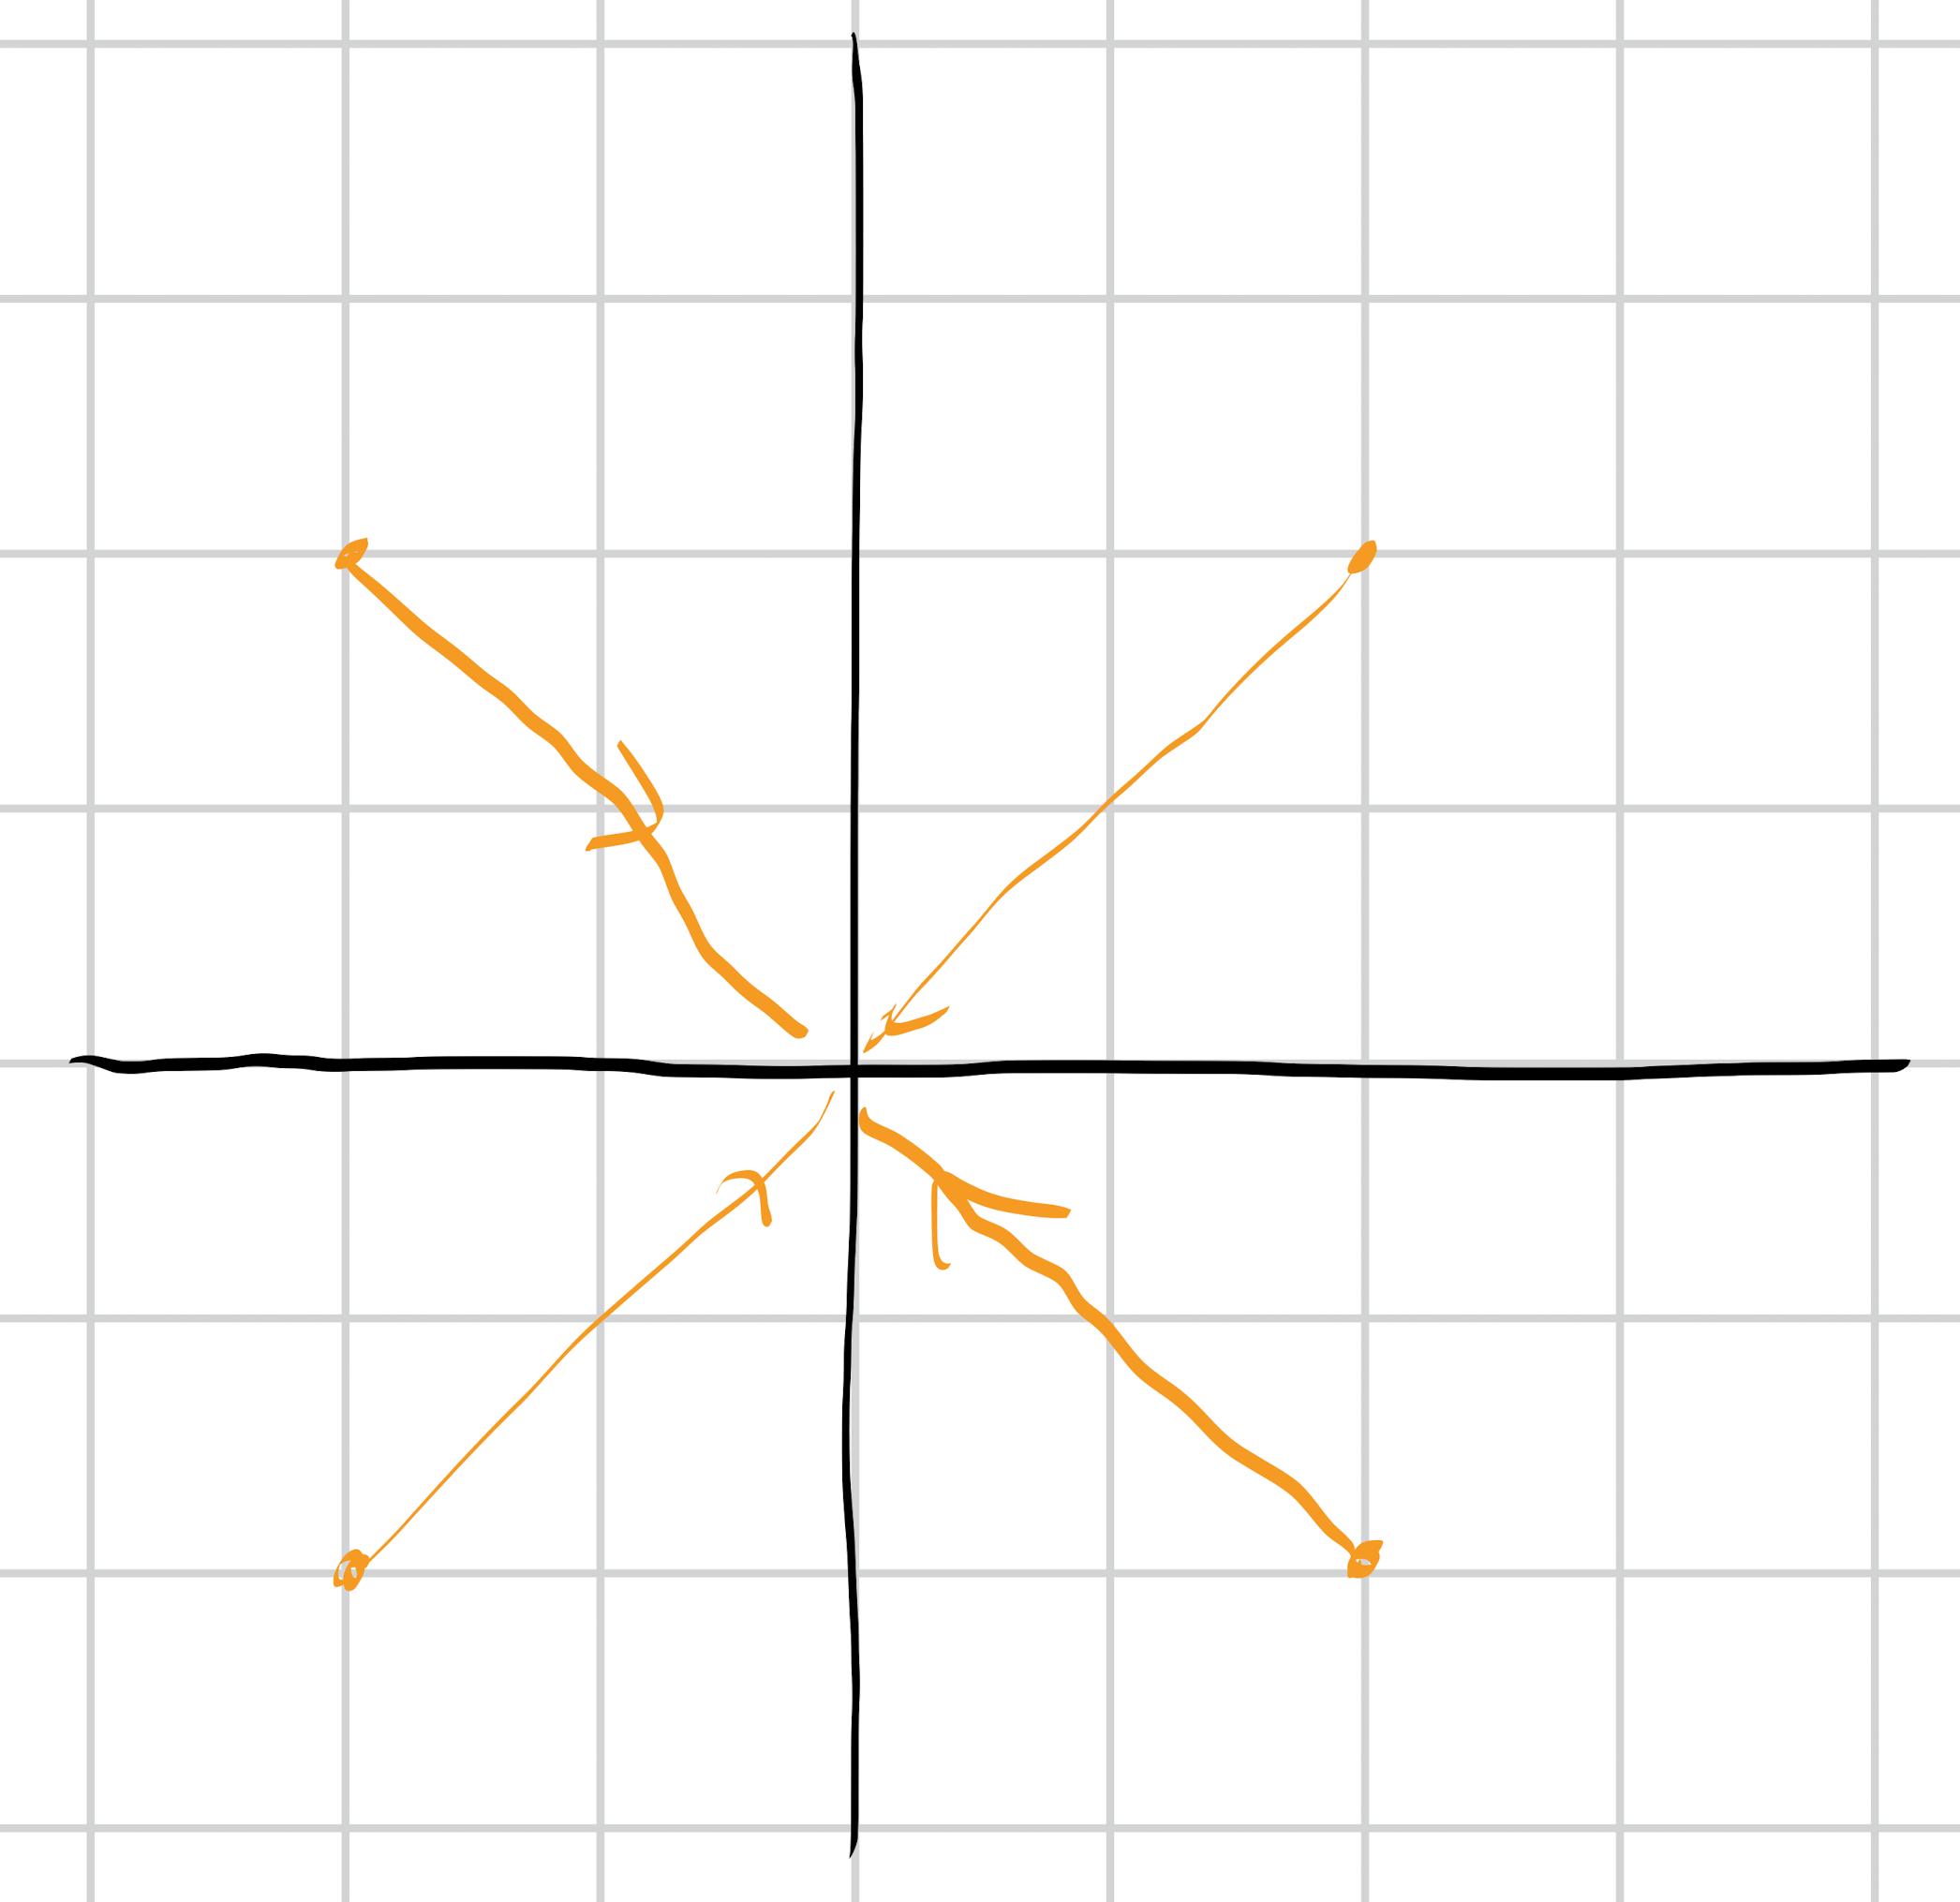
\includegraphics[width=10cm]{images/3_5_23c.png}
    \end{center}
  \item If $a = d > 0$, then the origin is a source star point. The general solution is
    \begin{align*}
      \vec{Y}(t) &= e^{at} \begin{pmatrix}x_0\\y_0\end{pmatrix}.
    \end{align*}
    Here, the eigenvector is the original condition. The phase portrait is as follows.
    \begin{center}
      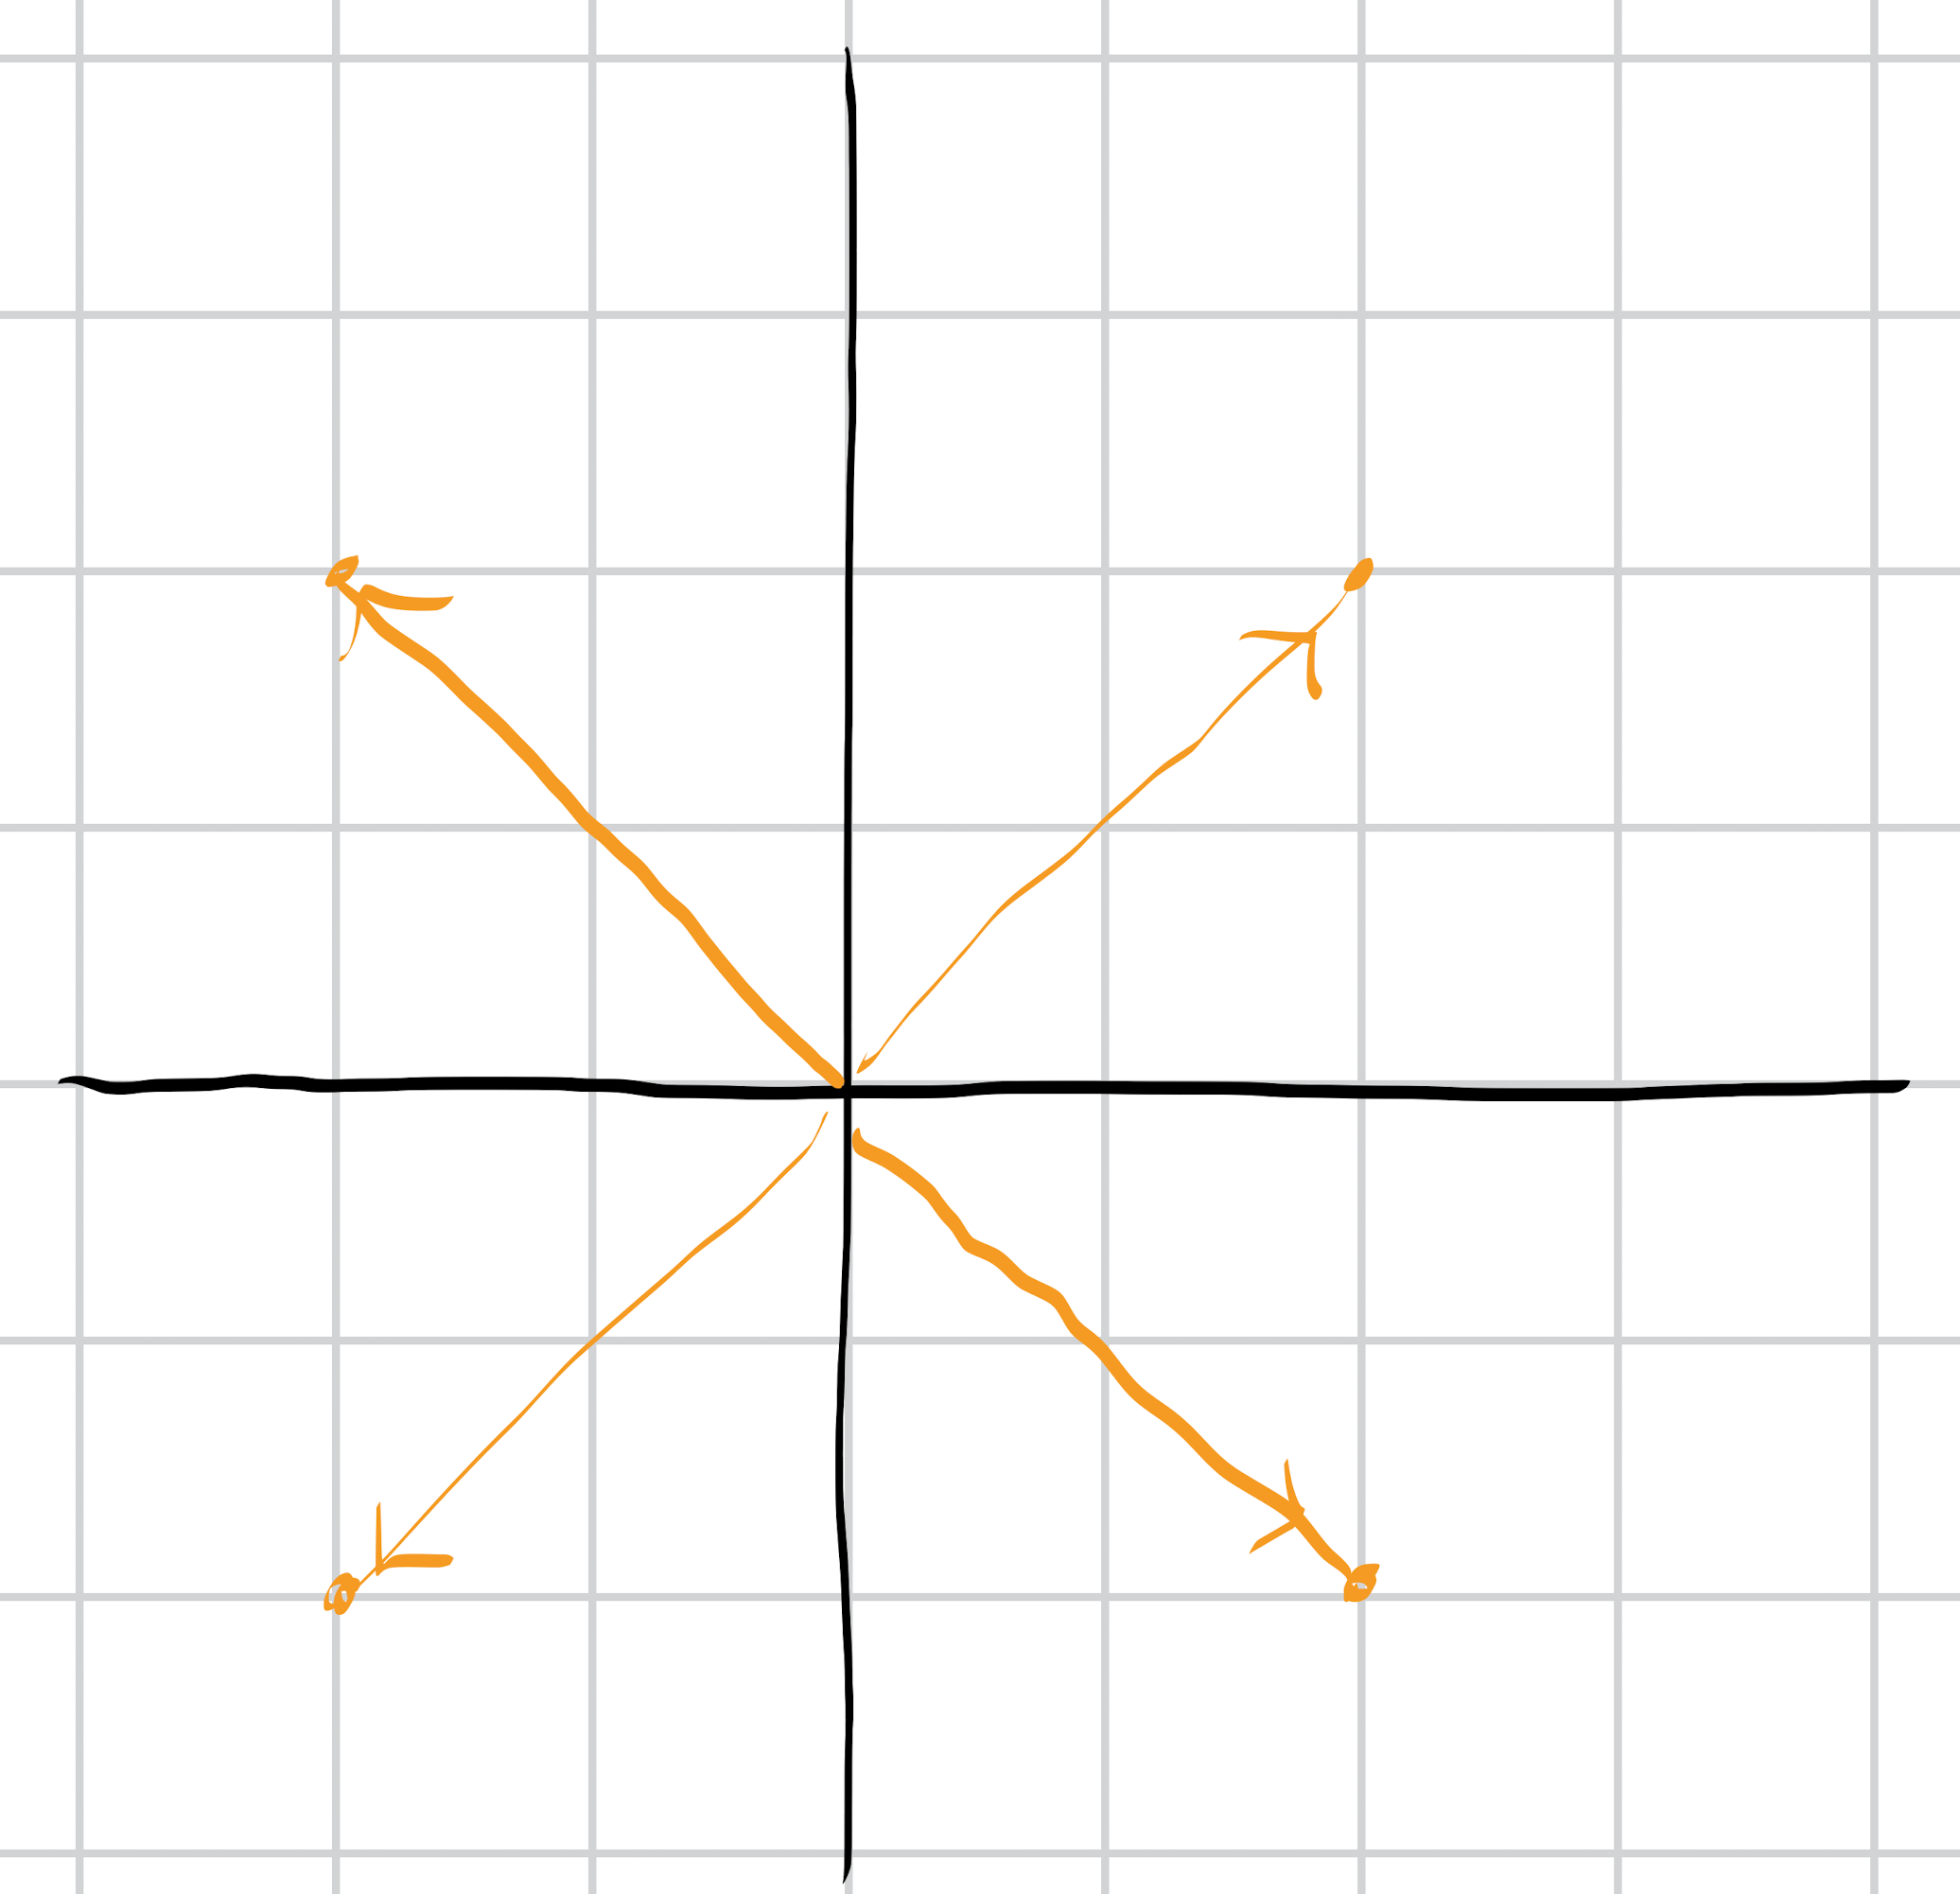
\includegraphics[width=10cm]{images/3_5_23d.png}
    \end{center}
\end{enumerate}
%\subsection{3.7, Problem 1}%
%I don't want to do this problem.
%\begin{description}[font=\normalfont\scshape]
%  \item[Saddle:]\hfill
%    \begin{itemize}
%      \item $\lambda_1,\lambda_2 \in \R$, $\lambda_1 > 0, \lambda_2 < 0$.
%      \item 
%        \begin{center}
%
%        \end{center}
%    \end{itemize}
%  \item[Attracting Fixed Points:]
%  \item[Sink:]
%  \item[Nodal Sink:]
%  \item[Spiral Sink:]
%  \item[Center:]
%  \item[Spiral Source:]
%  \item[Nodal Source:]
%  \item[Source:]
%  \item[Repelling Fixed Points:]
%\end{description}
\subsection{3.7, Problem 2}%
We see that $\tr(A) = a$ and $\det(A) = 2$.\newline
\begin{enumerate}[(a)]
  \item \hfill
    \begin{center}
      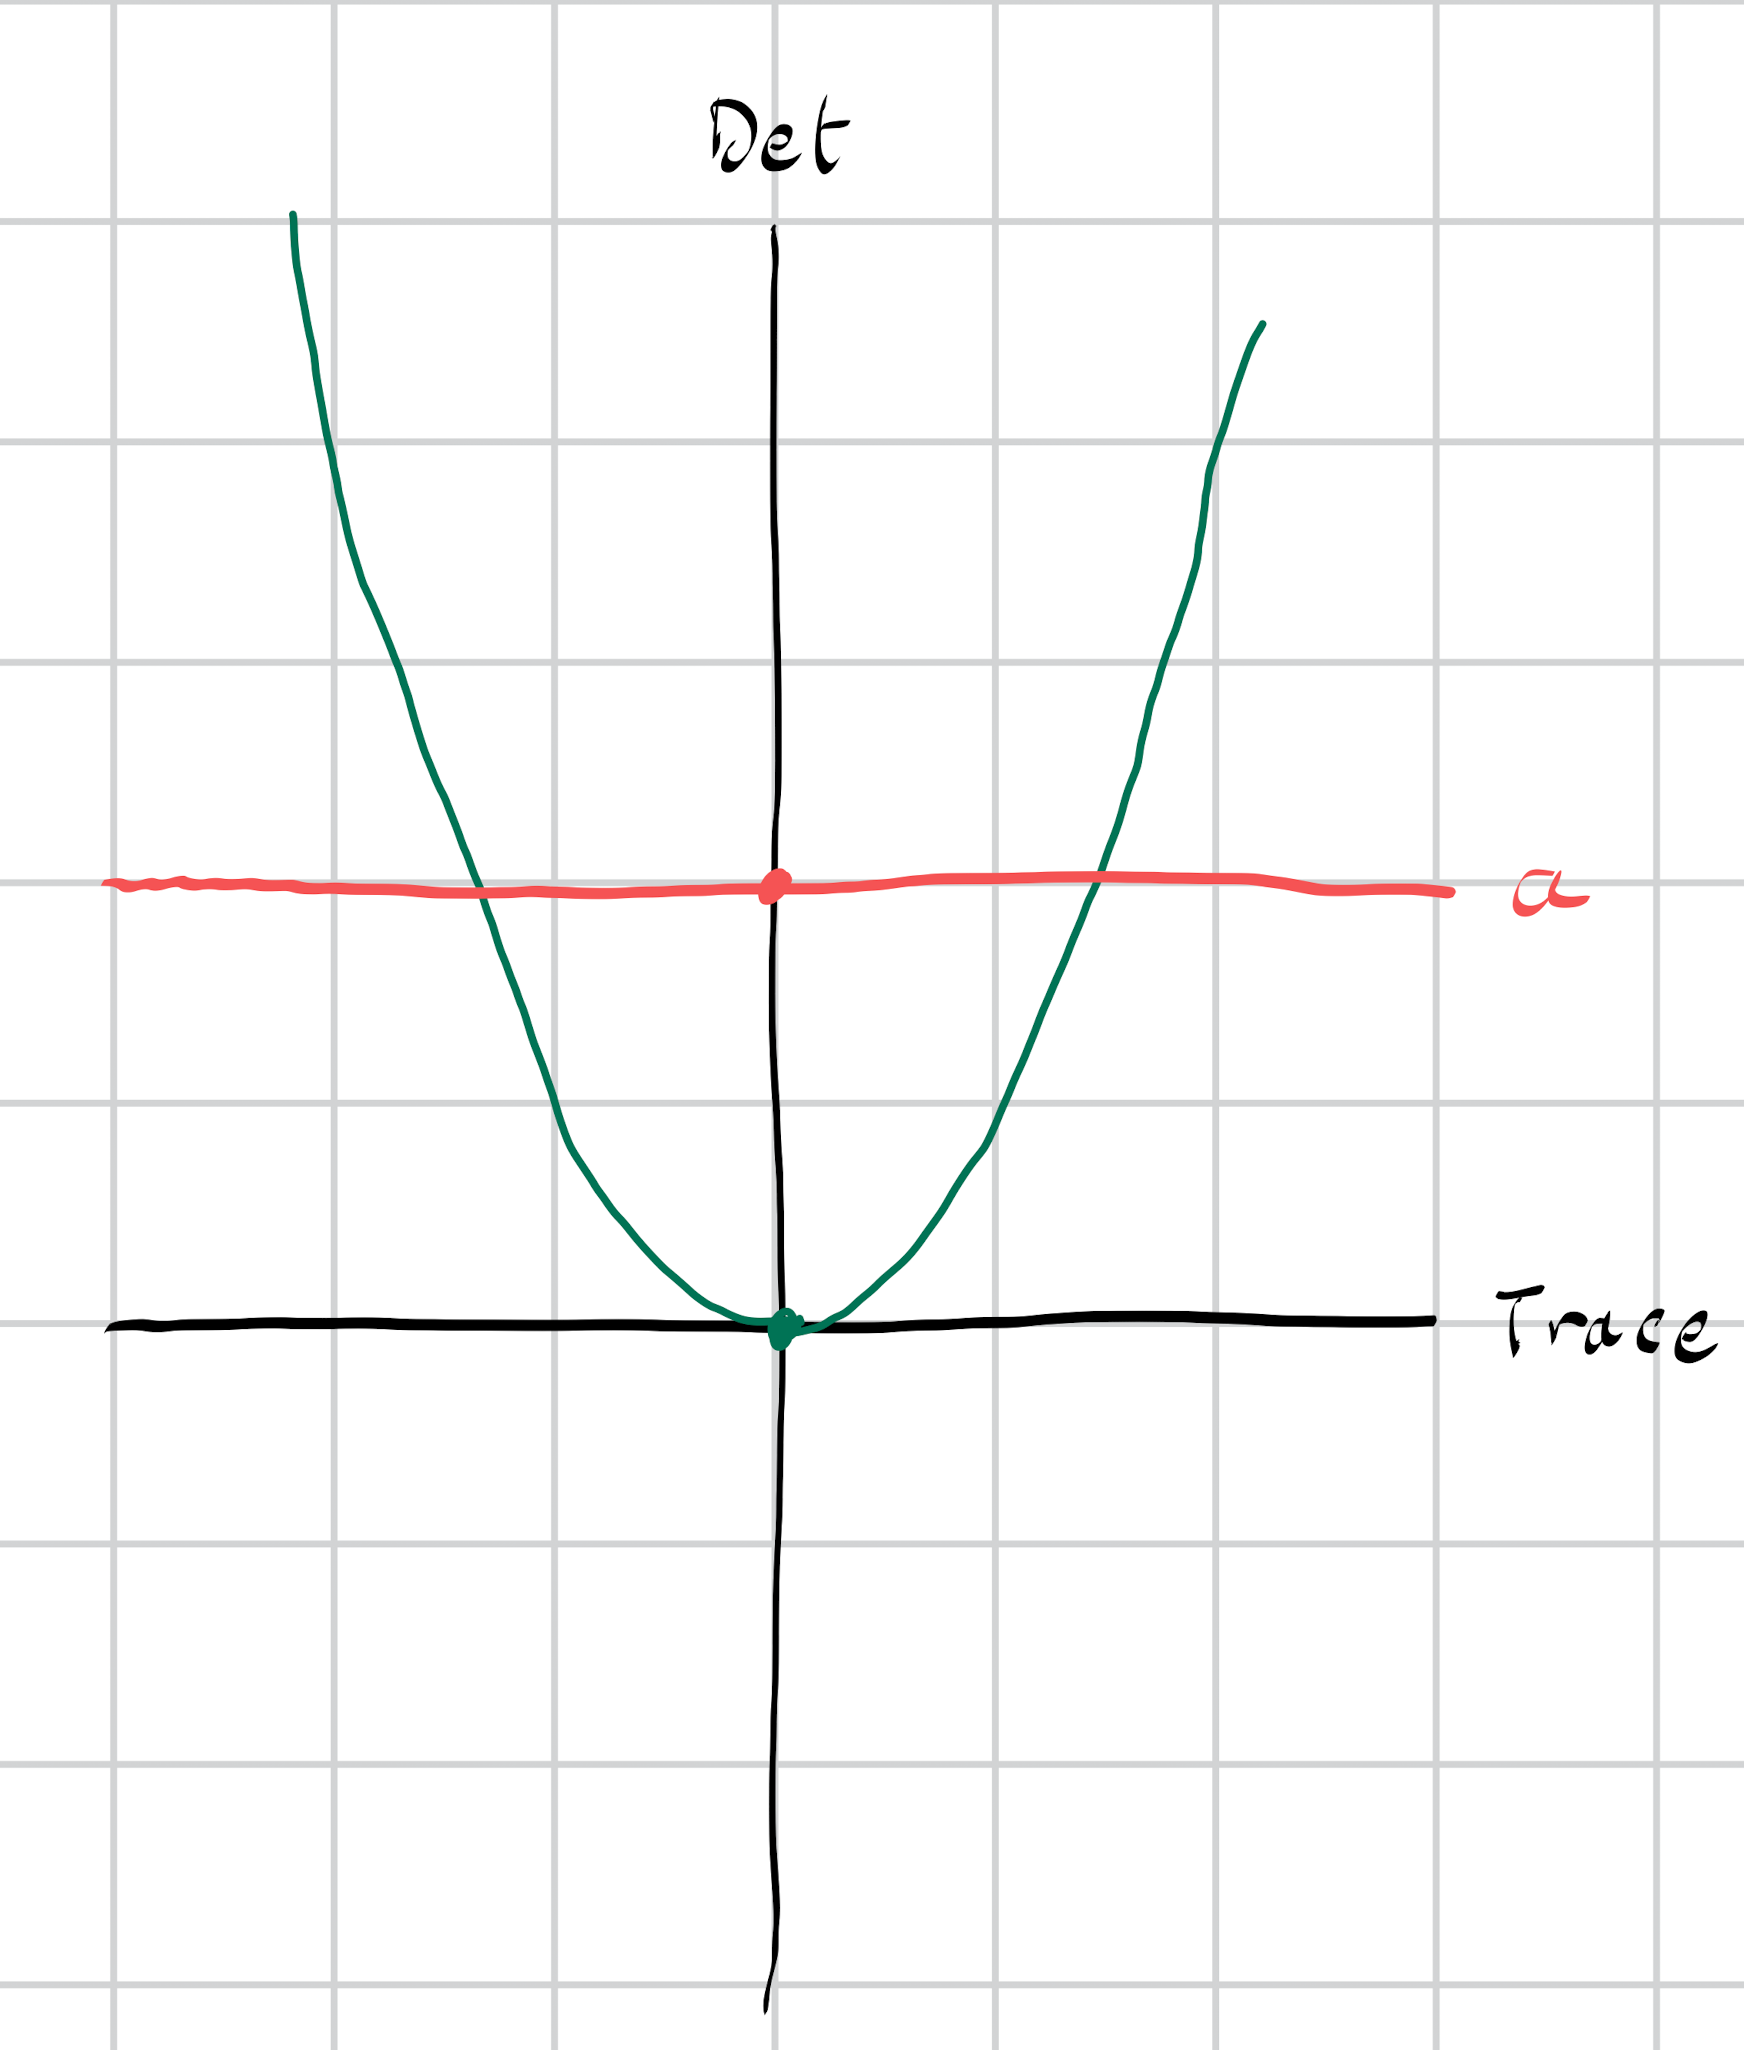
\includegraphics[width=7cm]{images/3_7_2a.png}
    \end{center}
  \item If $a < -\sqrt{2}$, we have a sink. If $-\sqrt{2} < a < 0$, we have a spiral sink. If $0 < a < \sqrt{2}$, we have a spiral source. If $a > \sqrt{2}$, we have a source. At $a = -\sqrt{2}$, we have a nodal sink, at $a = 0$, we have a center, and at $a = \sqrt{2}$, we have a nodal source.
  \item The bifurcation values are at $a = -\sqrt{2}$, $a = 0$, and at $a = \sqrt{2}$.
\end{enumerate}
\subsection{3.7, Problem 6}%
We see that $\tr(A) = -1$ and $\det(A) = -6$.
\begin{enumerate}[(a)]
  \item \hfill
    \begin{center}
      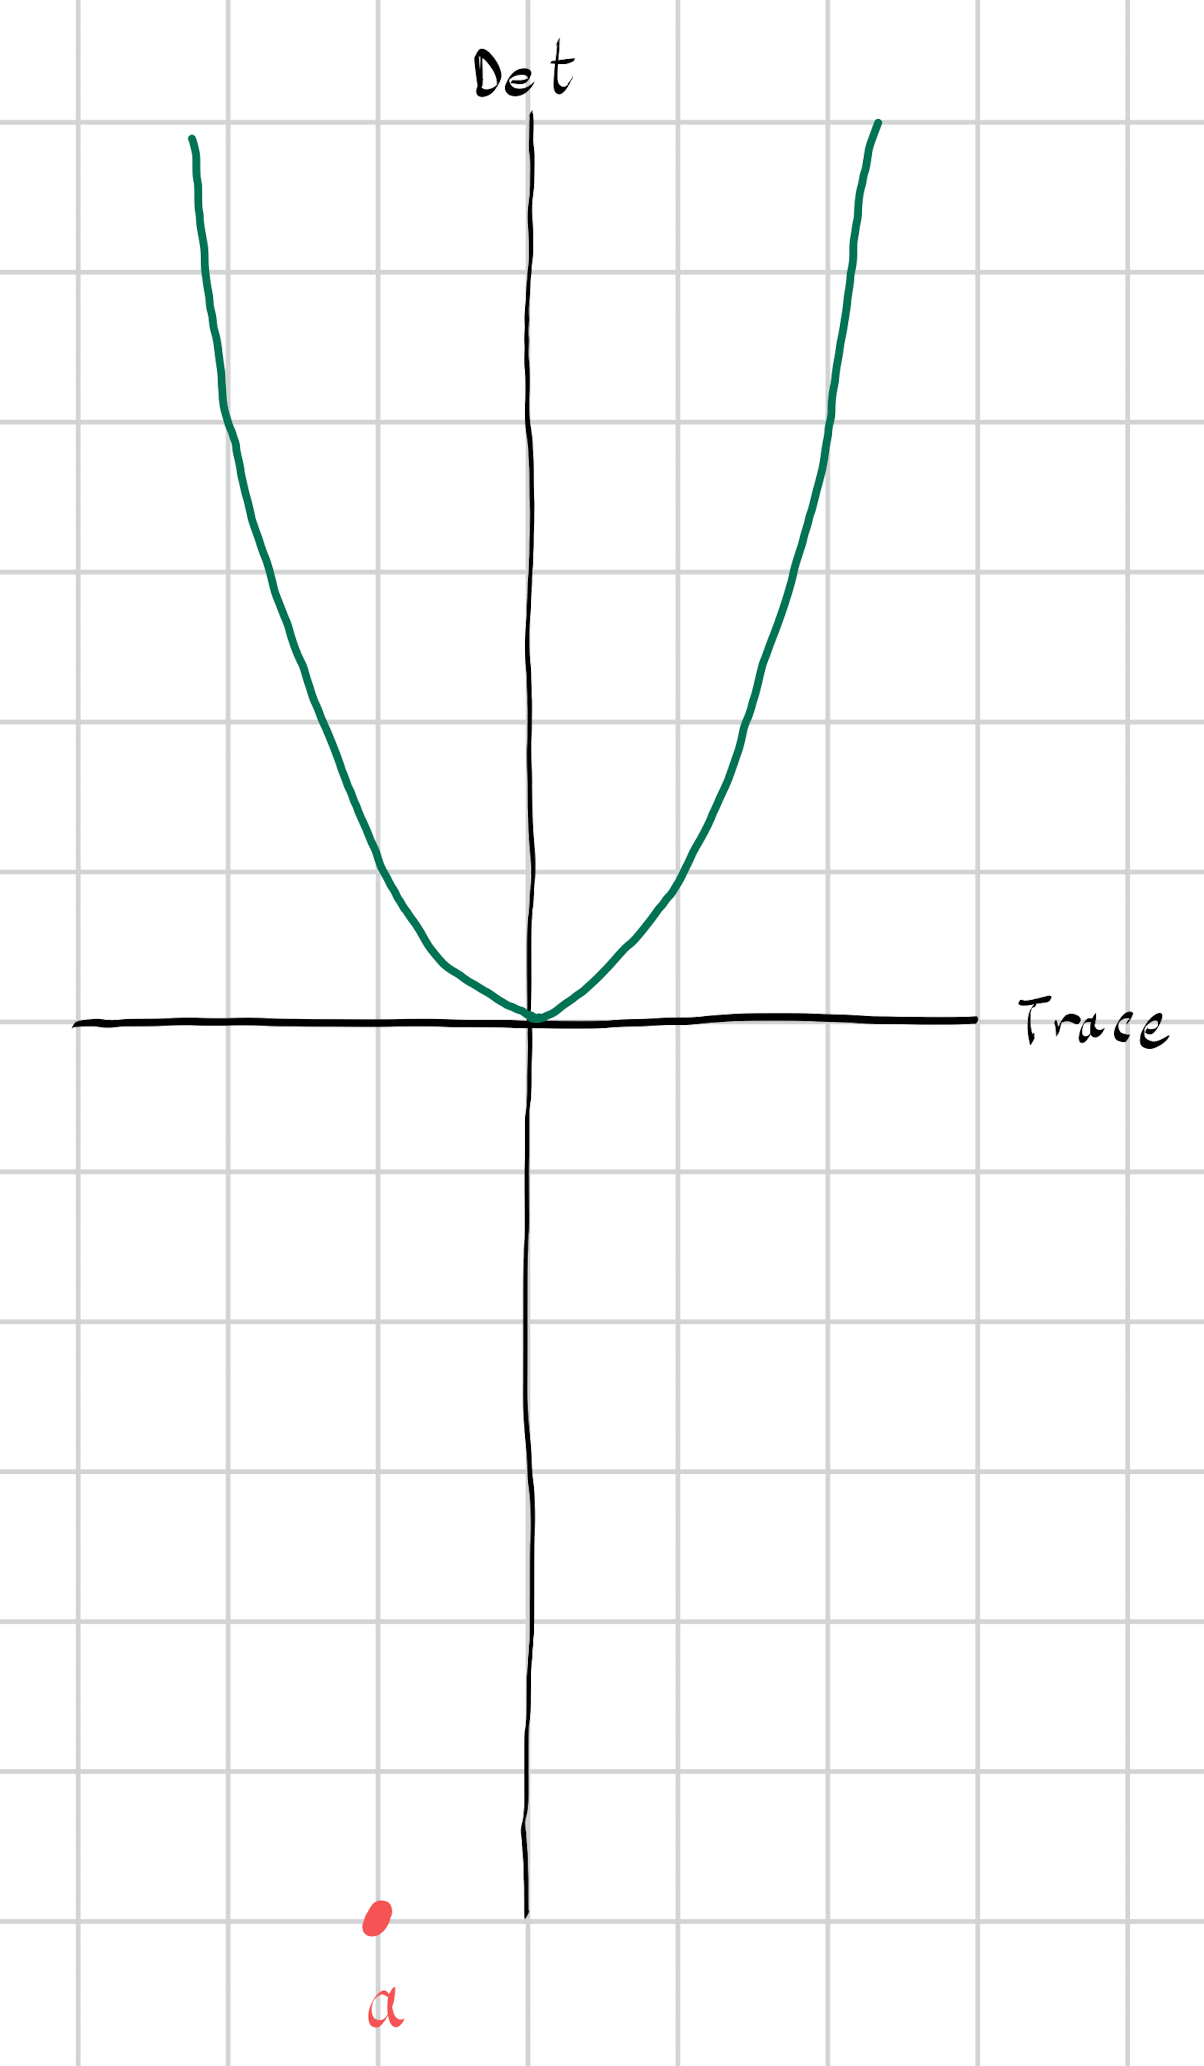
\includegraphics[width=7cm]{images/3_7_6a}
    \end{center}
  \item Since $a$ does not affect the parameter, we exclusively have a saddle.
  \item There are no bifurcation values for this system.
\end{enumerate}
\section{Part 2}%
\subsection{5.1, Problem 3}%
\begin{enumerate}[(a)]
  \item We start by finding the Jacobian
    \begin{align*}
      J &= \begin{pmatrix}-2 & 1 \\2x & -1 \end{pmatrix}\\
      J|_{(0,0)} &= \begin{pmatrix}-2 & 1 \\ 0 & -1\end{pmatrix},
    \end{align*}
    meaning the linearized system at $\left(0,0\right)$ is
    \begin{align*}
      \diff{\vec{U}}{t} &= \begin{pmatrix}-2 & 1 \\ 0 & -1\end{pmatrix} \vec{U}.
    \end{align*}
  \item The determinant is positive and the trace is negative, with $\det\left(A'\right) = 1$ and $\tr\left(A'\right) = -2$, so we have a nodal sink. The eigenvalue of this linearized system is at $\lambda = -1$, with corresponding eigenvector of $\vec{v} = \begin{pmatrix}1\\1\end{pmatrix}$.
  \item 
    \begin{center}
      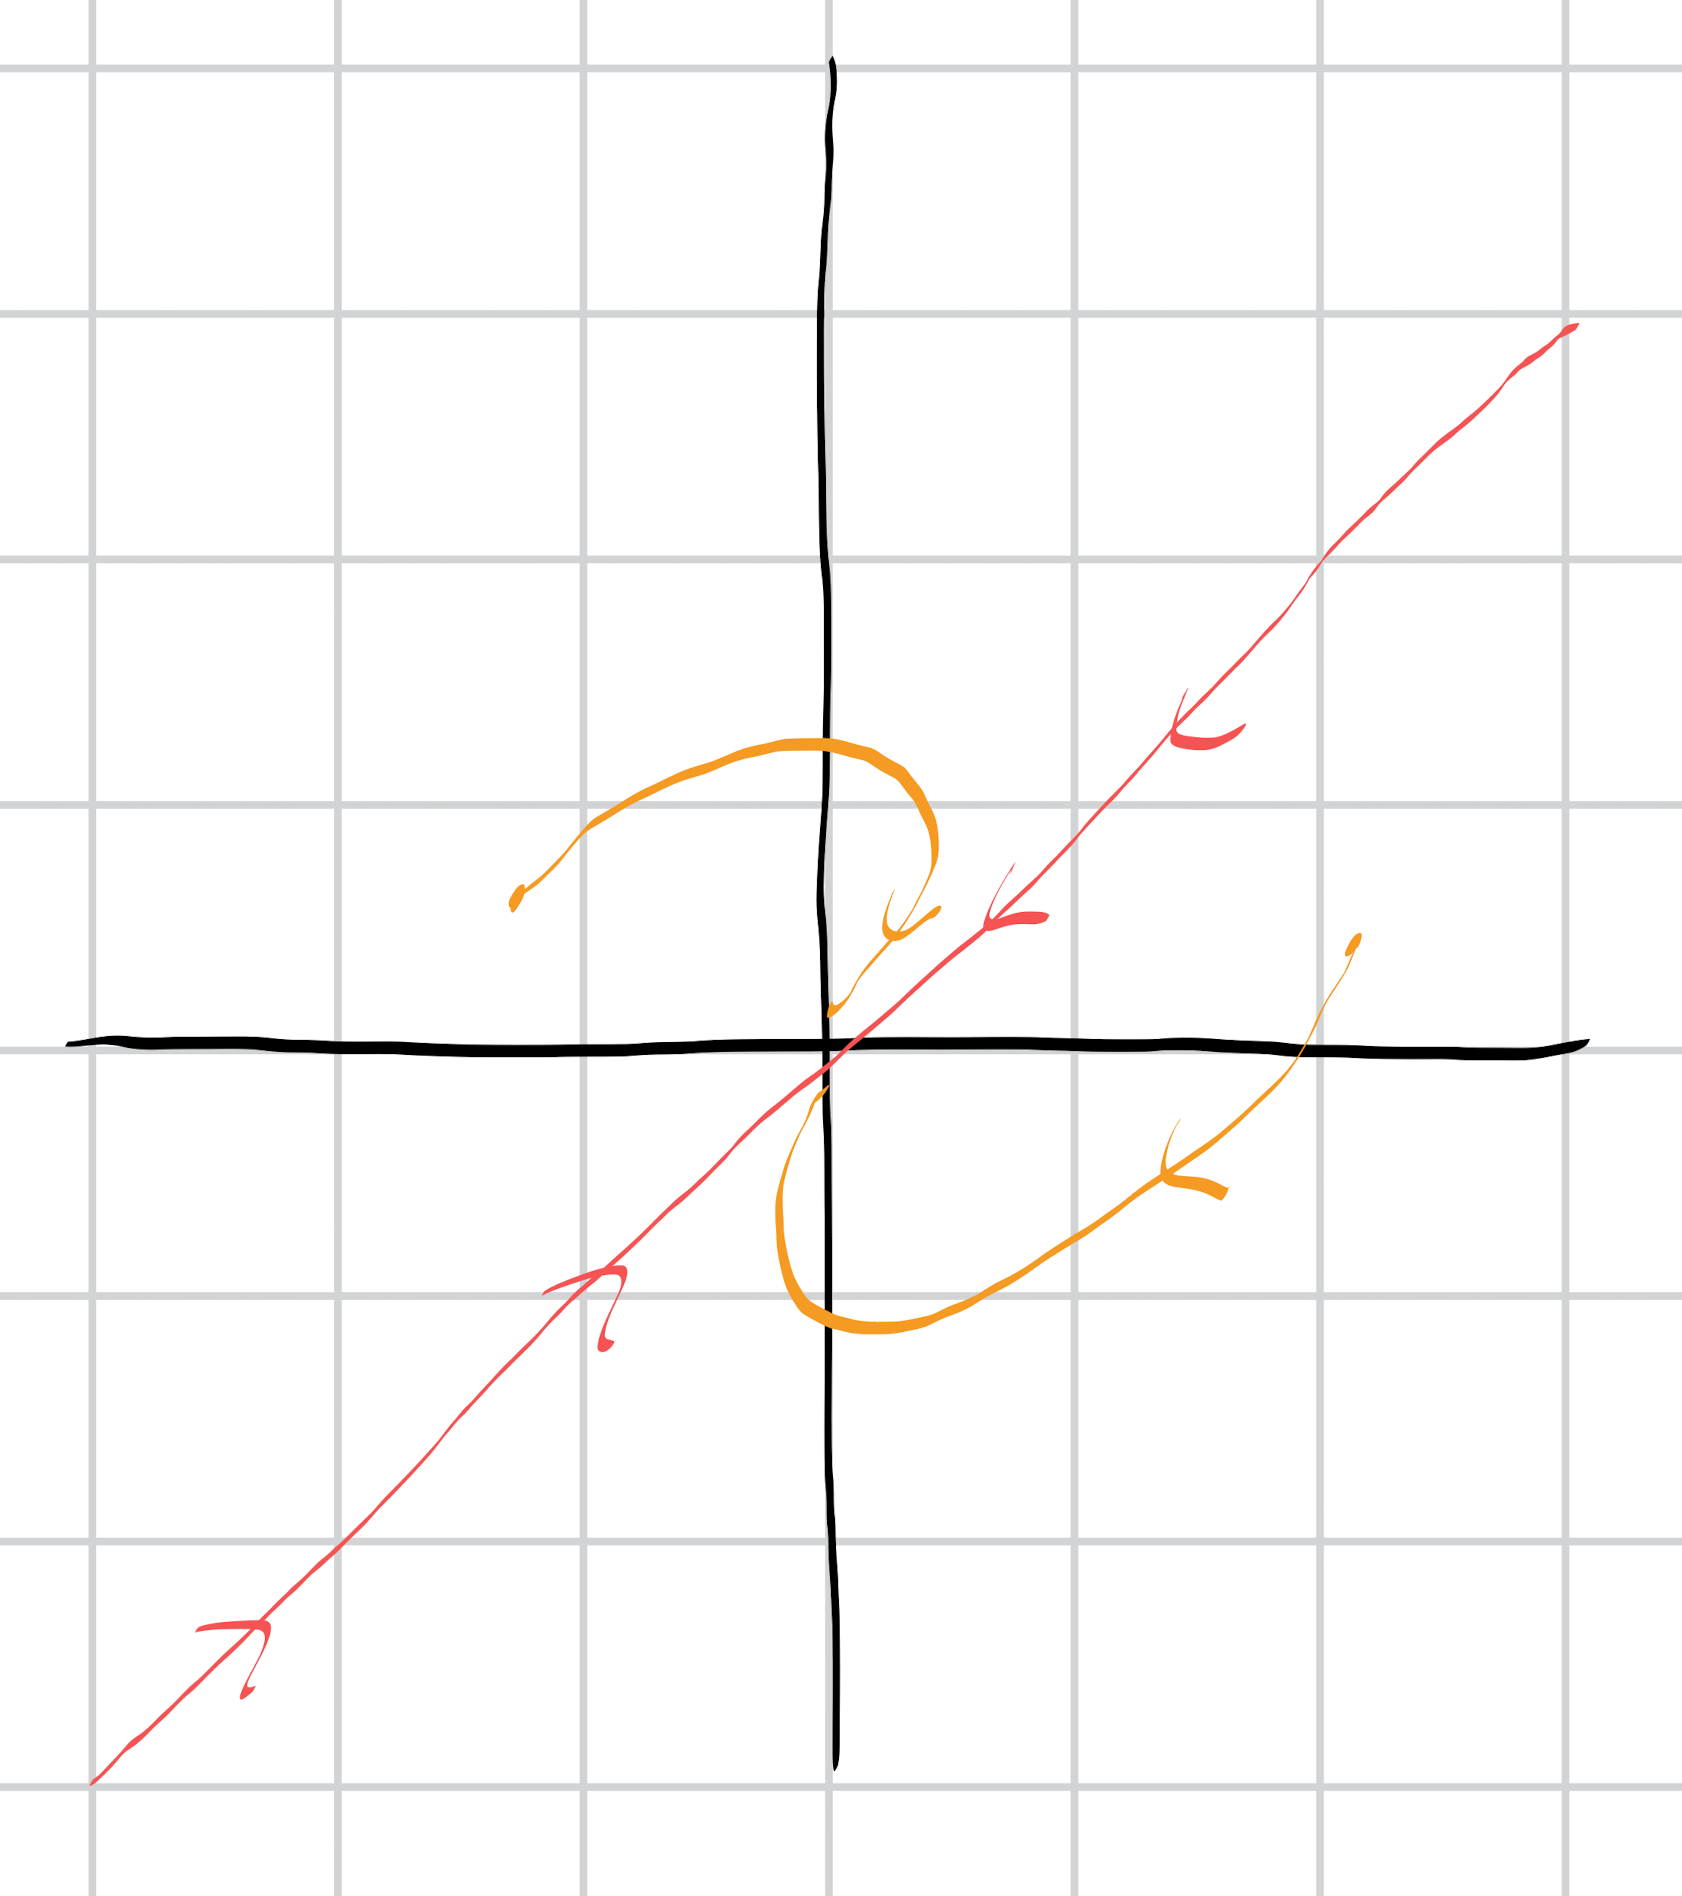
\includegraphics[width=7cm]{images/5_1_3c1.png}
    \end{center}
  \item 
    \begin{enumerate}[(a)]
      \item The Jacobian evaluated at $\left(2,4\right)$ is
        \begin{align*}
          J|_{\left(2,4\right)} &= \begin{pmatrix}-2 & 1 \\ 4 & -1\end{pmatrix}
        \end{align*}
      \item The trace and determinant are both negative, so this is a saddle.
      \item 
        \begin{center}
          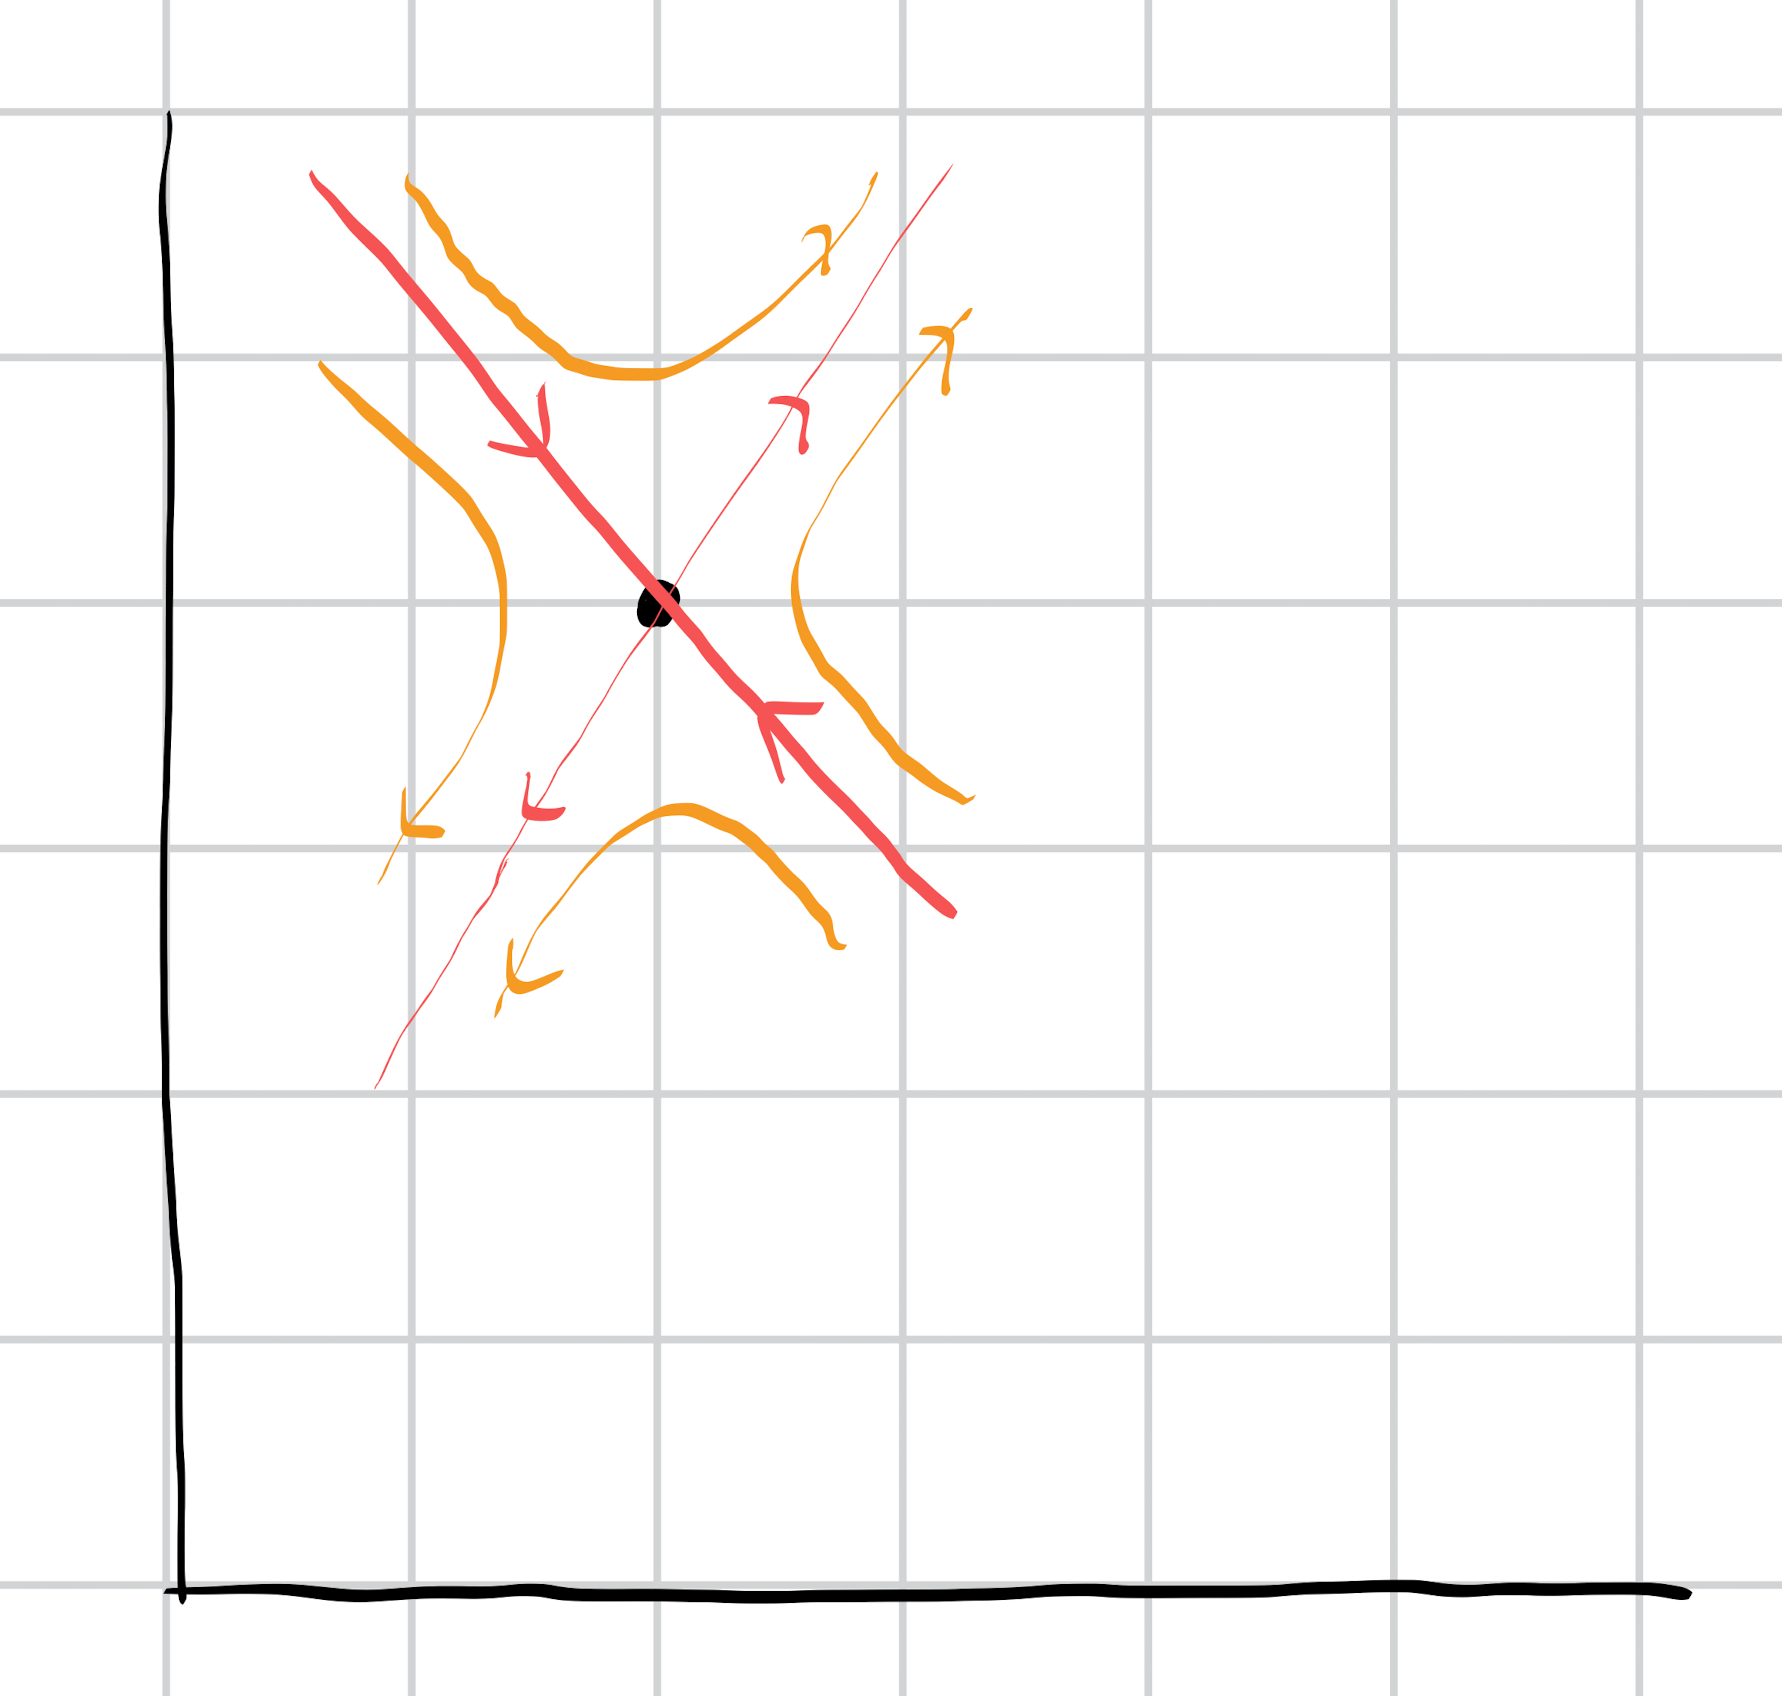
\includegraphics[width=7cm]{images/5_1_3c2.png}
        \end{center}
    \end{enumerate}
\end{enumerate}
\subsection{5.1, Problem 4}%
\begin{enumerate}[(a)]
  \item Since $\diff{x}{t} = 0$ if and only if $-x = 0$, we have that $\diff{y}{t} = 0$ if and only if $y = 0$. Thus $\left(0,0\right)$ is the only equilibrium point.
  \item Taking partial derivatives, we have the linearized system
    \begin{align*}
      \diff{\vec{U}}{t} &= \begin{pmatrix}-1 & 0 \\ 0 & 1\end{pmatrix}.
    \end{align*}
  \item The linearized system is a saddle with eigenvectors of $ \begin{pmatrix}1\\0\end{pmatrix} $ and $ \begin{pmatrix}0\\1\end{pmatrix} $.
\end{enumerate}
\subsection{5.1, Problem 5}%
\begin{enumerate}[(a)]
  \item The general solution to $\diff{x}{t} = -x$ is $k_1e^{-t}$.
  \item Substituting, we have
    \begin{align*}
      \diff{y}{t} &= -4k_1e^{-3t} + y\\
      \diff{y}{t} - y &= -4k_1e^{-3t}\\
      e^{-t}\diff{y}{t} - e^{-t}y &= -4k_1e^{-4t}\\
      \diff{}{t}\left(e^{-t}y\right) &= -4k_1e^{-4t}\\
      y &= k_1e^{-3t} + k_2e^{t}.
    \end{align*}
  \item The general solution is
    \begin{align*}
      \vec{Y}_1(t) &= \begin{pmatrix}k_1e^{-3t} \\ k_1e^{-3t} + k_2e^{t}\end{pmatrix}.
    \end{align*}
  \item The solution curves that tend toward the origin as $t\rightarrow\infty$ are all the ones that have $k_2 = 0$.
  \item The solution curves that tend toward the origin as $t\rightarrow -\infty$ are all the ones that have $k_1 = 0$.
  \item 
    \begin{center}
      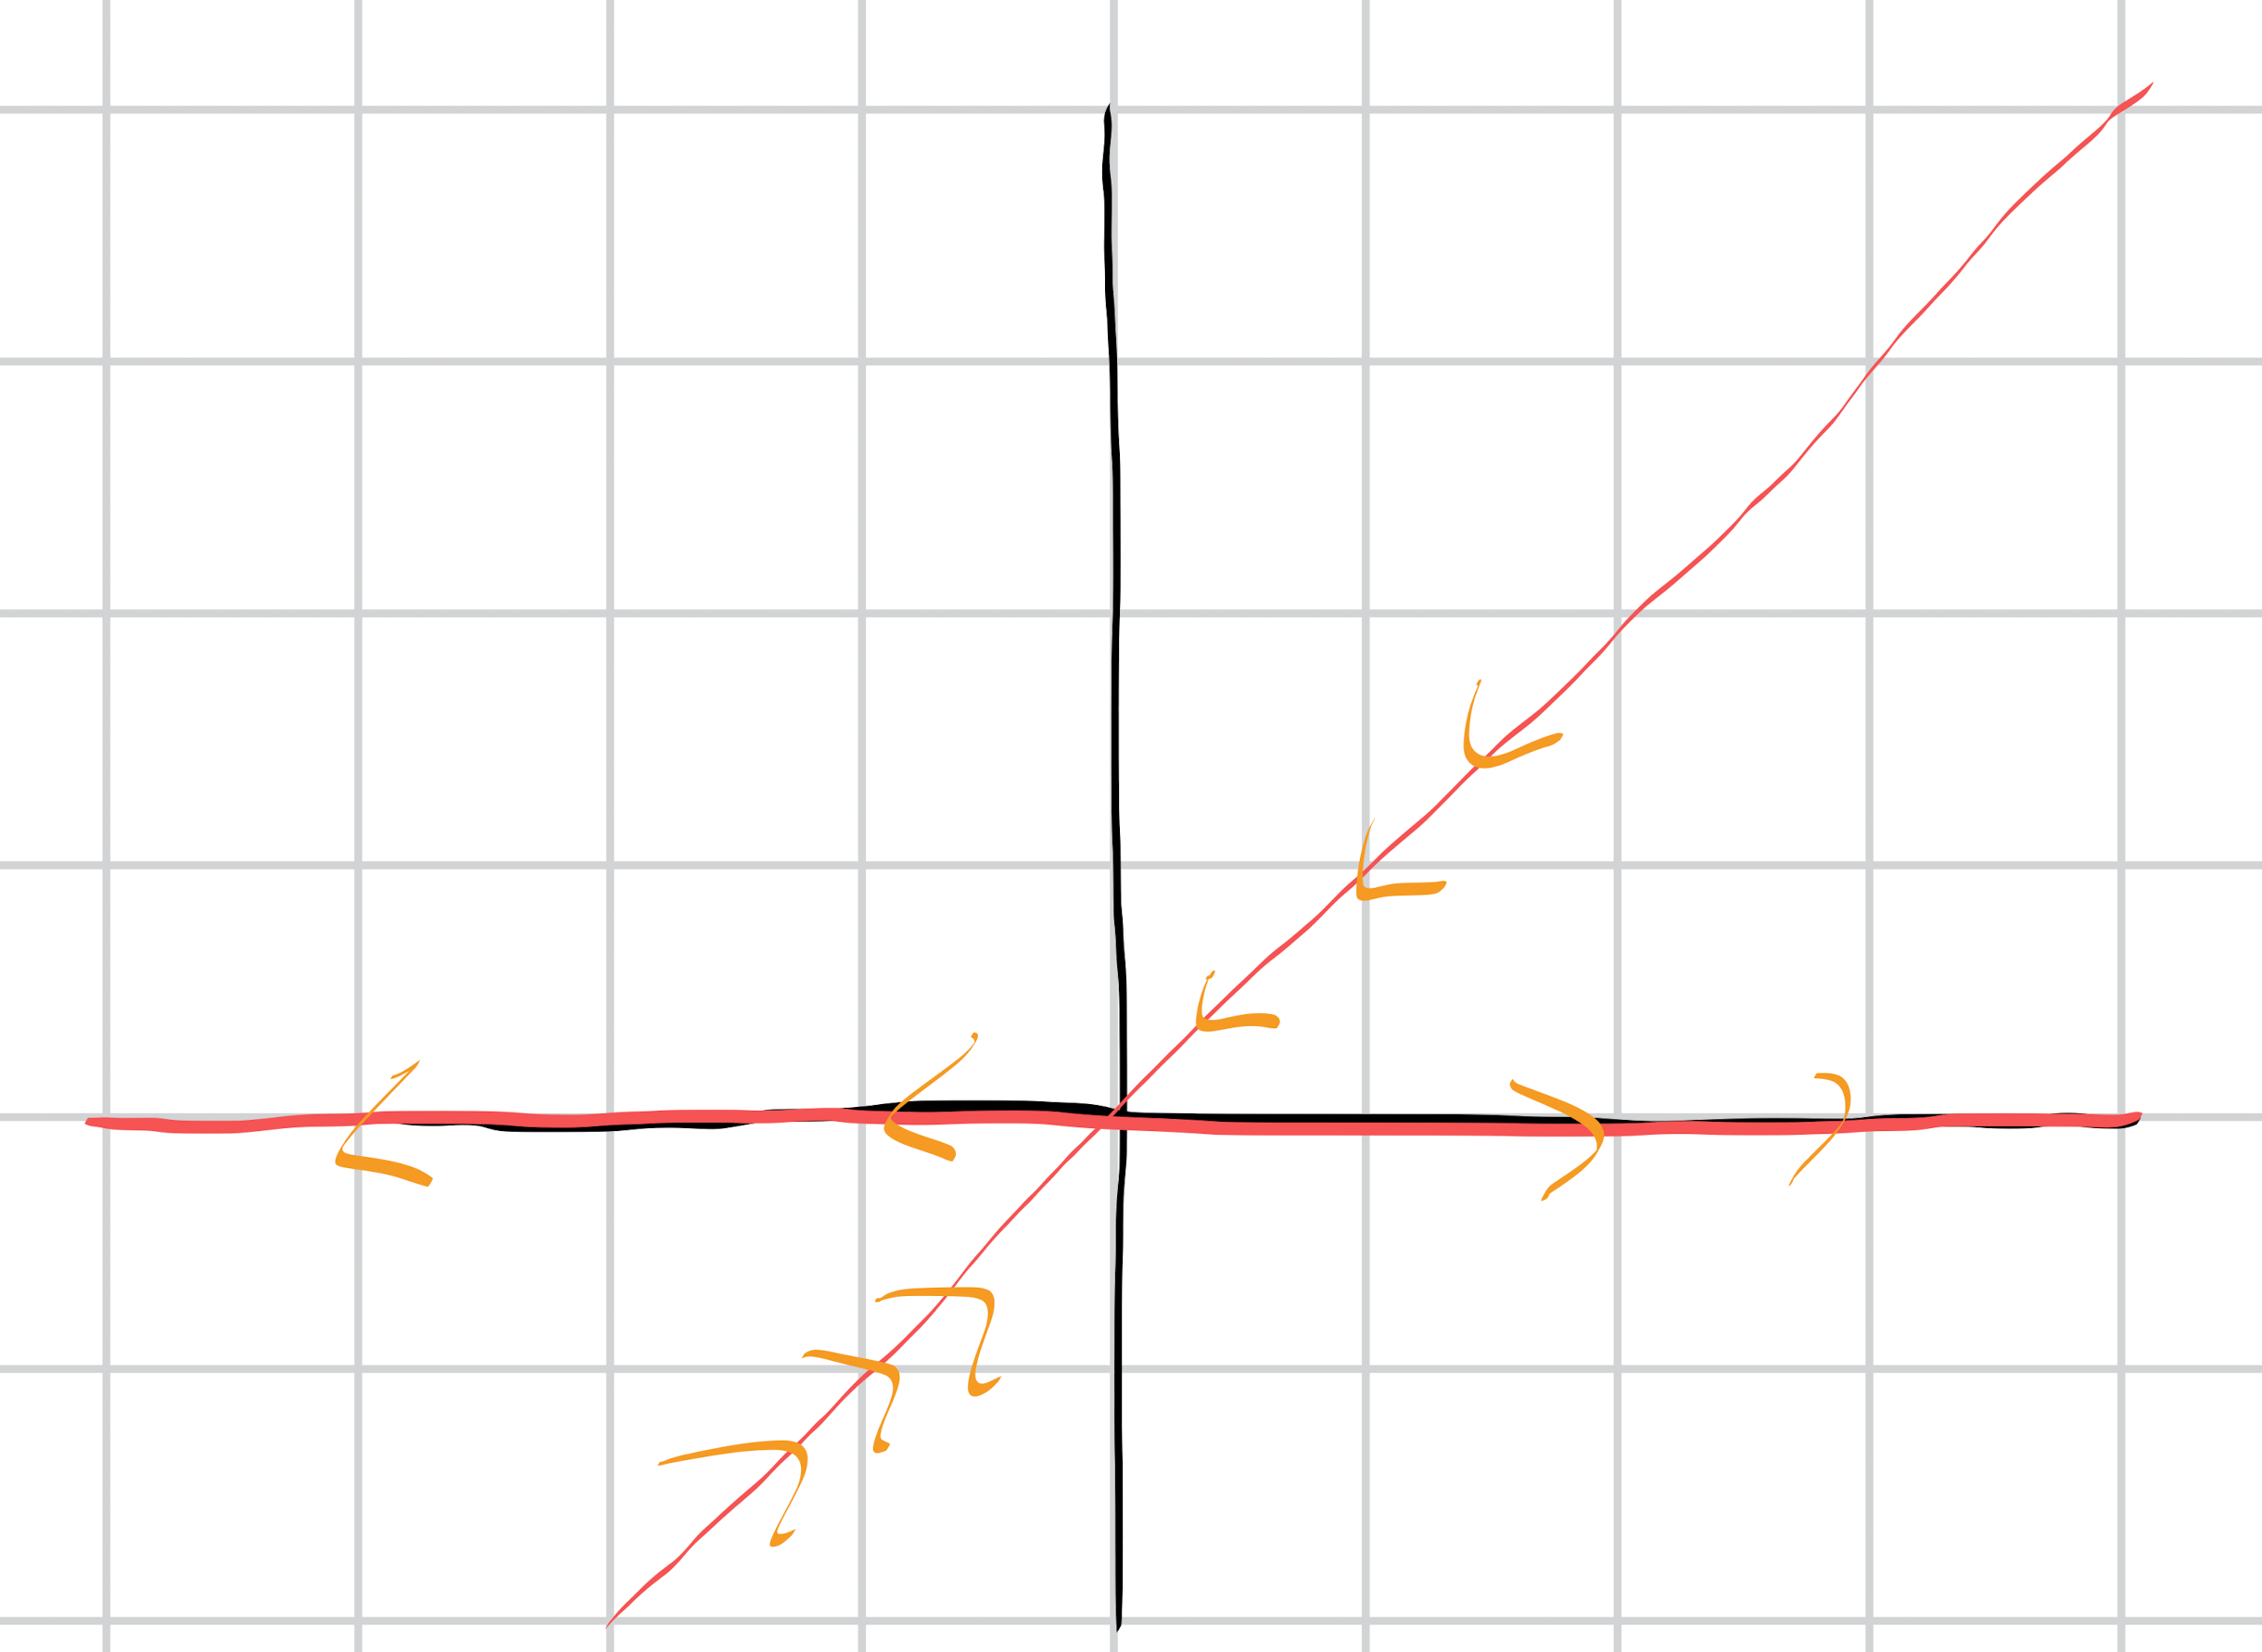
\includegraphics[width=10cm]{images/5_1_5f.png}
    \end{center}
  \item The linearized system and the separatrix solutions appear very similar, albeit that the vectors along which the solution curves tend to zero are different than the phase portrait of the linearized system.
\end{enumerate}
\subsection{5.1, Problem 8}%
\begin{enumerate}[(a)]
  \item We find the Jacobian to be
    \begin{align*}
      J &= \begin{pmatrix}-2x + 10 - y & -x \\ 2y & -2x - 2y + 30\end{pmatrix}.
    \end{align*}
    The equilibrium points are at $\left(0,0\right)$, $\left(10,0\right)$, $\left(0,30\right)$, $\left(20,-10\right)$. The respective Jacobians are
    \begin{align*}
      J|_{(0,0)} &= \begin{pmatrix}10 & 0 \\ 0 & 30\end{pmatrix}\\
      J|_{(10,0)} &= \begin{pmatrix}-10 & -10 \\ 0 & 10\end{pmatrix}\\
      J|_{(0,30)} &= \begin{pmatrix}-20 & 0 \\ 60 & -30\end{pmatrix}\\
      J|_{(20,-10)} &= \begin{pmatrix}-20 & -20 \\ -20 & 10\end{pmatrix}.
    \end{align*}
    \begin{itemize}
      \item The equilibrium point at $\left(0,0\right)$ is a source.
      \item The equilibrium point at $\left(10,0\right)$ is a saddle.
      \item The equilibrium point at $\left(0,30\right)$ is a nodal sink.
      \item The equilibrium point at $\left(20,-10\right)$ is a spiral sink.
    \end{itemize}
\end{enumerate}
\subsection{5.1, Problem 18}%
\begin{enumerate}[(a)]
  \item If $a < 0$, then $\diff{x}{t} = x^2 - a$ is always greater than zero, so $\diff{x}{t}$ is never zero.
  \item If $ a > 0 $, then $\diff{x}{t} = x^2 - a$ is zero when $x = \pm \sqrt{a}$. Since $x^2 + 1$ is always greater than zero, $\diff{y}{t} = 0$ only when $y = 0$, so there are two equilibrium points at $x = \pm \sqrt{a},y=0$.
  \item If $ a = 0 $, then the only equilibrium point is at $\left(0,0\right)$, as $\diff{x}{t} = 0$ only when $x = 0$ and $\diff{y}{t} = 0$ only when $y = 0$.
  \item The linearization at $ a = 0 $ is
    \begin{align*}
      J|_{(0,0)} &= \begin{pmatrix}0 & 0 \\ 0 & -1\end{pmatrix},
    \end{align*}
    The eigenvalues are $\lambda = 0$ and $\lambda = -1$.
\end{enumerate}
\subsection{5.1, Problem 20}%
\begin{enumerate}[(a)]
  \item The equilibrium point for $y$ occurs at $y = a$, so for $a > 0$ we have equilibrium points at $\left(-\sqrt{a},a\right), \left(\sqrt{a},a\right)$; if $a = 0$, then the equilibrium point is at $\left(0,0\right)$, and if $a < 0$, there is no equilibrium point.
  \item The bifurcation occurs at $a = 0$.
  \item For $a < 0$, there are no equilibrium points, and at $a = 0$, there is a line of repelling fixed points. At $\left(-\sqrt{a},a\right)$, there is a saddle point, and at $\left(\sqrt{a},a\right)$ there is either a spiral source (as depicted below) or a source, depending on the value of $a$.
    \begin{center}
      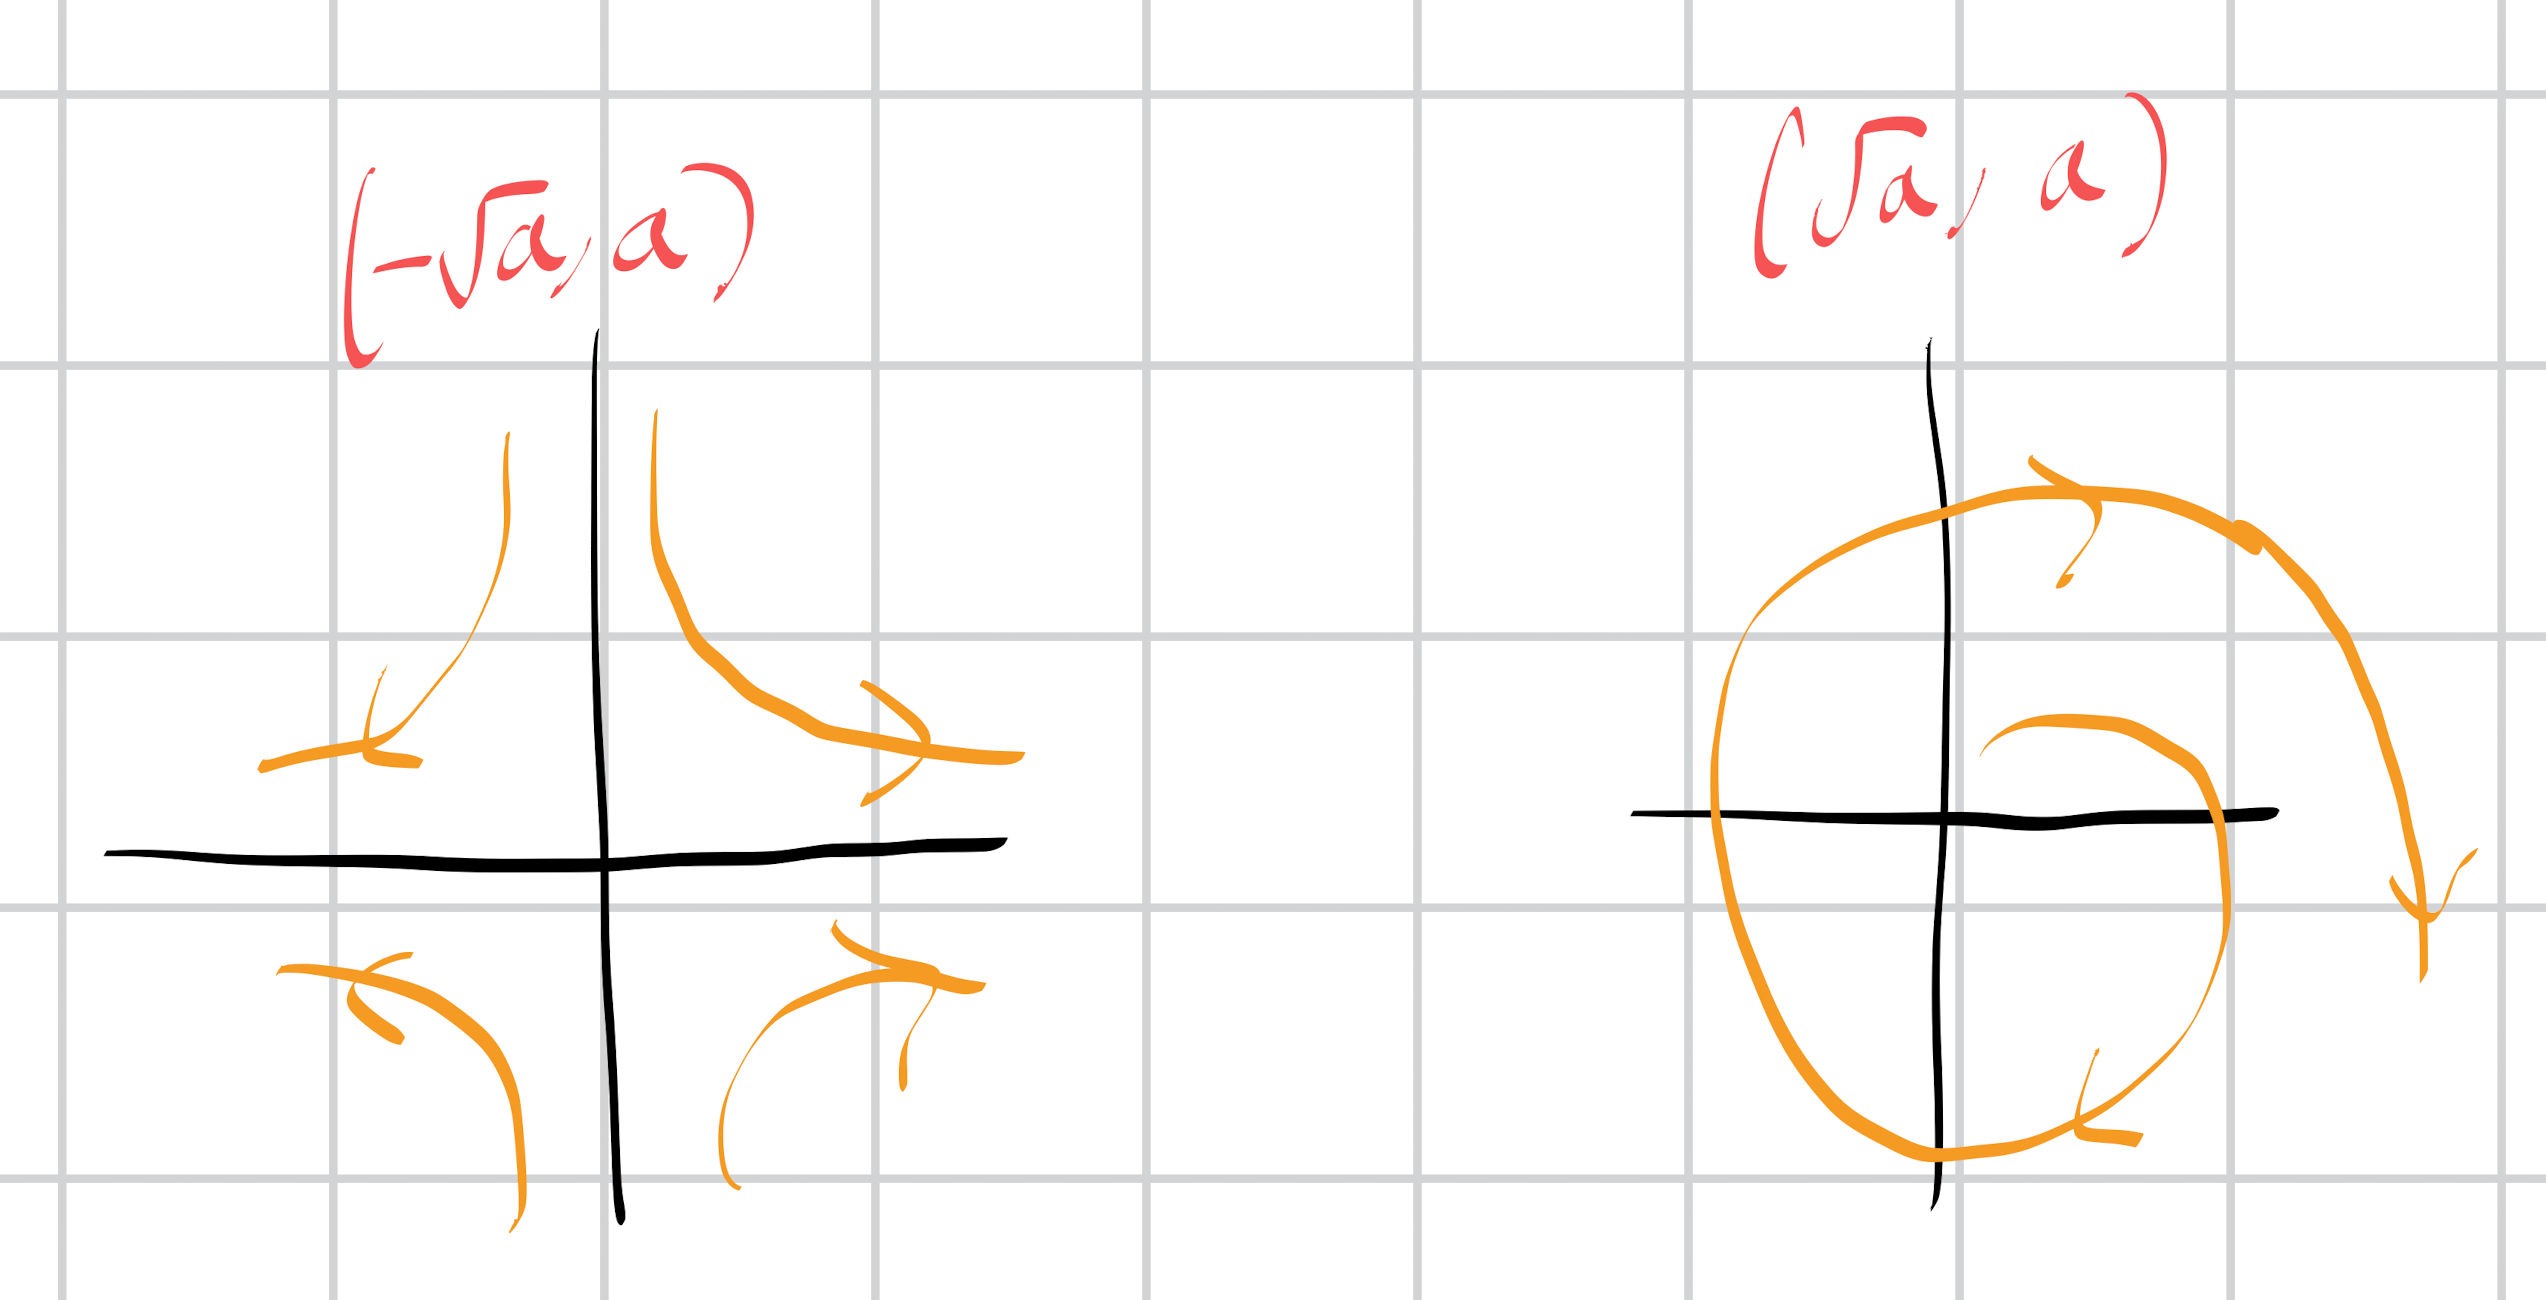
\includegraphics[width=10cm]{images/5_1_20c.png}
    \end{center}
\end{enumerate}
\end{document}
